%  LaTeX support: latex@mdpi.com 
%  For support, please attach all files needed for compiling as well as the log file, and specify your operating system, LaTeX version, and LaTeX editor.

%=================================================================
\documentclass[jmse,review,submit,pdftex,moreauthors]{Definitions/mdpi}
%\documentclass[preprints,article,submit,pdftex,moreauthors]{Definitions/mdpi} 
% For posting an early version of this manuscript as a preprint, you may use "preprints" as the journal. Changing "submit" to "accept" before posting will remove line numbers.

% Below journals will use APA reference format:
% admsci, behavsci, businesses, econometrics, economies, education, ejihpe, famsci, games, humans, ijcs, ijfs, journalmedia, jrfm, languages, psycholint, publications, tourismhosp, youth

% Below journals will use Chicago reference format:
% arts, genealogy, histories, humanities, jintelligence, laws, literature, religions, risks, socsci

%--------------------
% Class Options:
%--------------------
%----------
% journal
%----------
% Choose between the following MDPI journals:
% accountaudit, acoustics, actuators, addictions, adhesives, admsci, adolescents, aerobiology, aerospace, agriculture, agriengineering, agrochemicals, agronomy, ai, air, algorithms, allergies, alloys, amh, analytica, analytics, anatomia, anesthres, animals, antibiotics, antibodies, antioxidants, applbiosci, appliedchem, appliedmath, appliedphys, applmech, applmicrobiol, applnano, applsci, aquacj, architecture, arm, arthropoda, arts, asc, asi, astronomy, atmosphere, atoms, audiolres, automation, axioms, bacteria, batteries, bdcc, behavsci, beverages, biochem, bioengineering, biologics, biology, biomass, biomechanics, biomed, biomedicines, biomedinformatics, biomimetics, biomolecules, biophysica, biosensors, biosphere, biotech, birds, blockchains, bloods, blsf, brainsci, breath, buildings, businesses, cancers, carbon, cardiogenetics, catalysts, cells, ceramics, challenges, chemengineering, chemistry, chemosensors, chemproc, children, chips, cimb, civileng, cleantechnol, climate, clinbioenerg, clinpract, clockssleep, cmd, cmtr, coasts, coatings, colloids, colorants, commodities, complications, compounds, computation, computers, condensedmatter, conservation, constrmater, cosmetics, covid, crops, cryo, cryptography, crystals, csmf, ctn, curroncol, cyber, dairy, data, ddc, dentistry, dermato, dermatopathology, designs, devices, diabetology, diagnostics, dietetics, digital, disabilities, diseases, diversity, dna, drones, dynamics, earth, ebj, ecm, ecologies, econometrics, economies, education, eesp, ejihpe, electricity, electrochem, electronicmat, electronics, encyclopedia, endocrines, energies, eng, engproc, ent, entomology, entropy, environments, epidemiologia, epigenomes, esa, est, famsci, fermentation, fibers, fintech, fire, fishes, fluids, foods, forecasting, forensicsci, forests, fossstud, foundations, fractalfract, fuels, future, futureinternet, futureparasites, futurepharmacol, futurephys, futuretransp, galaxies, games, gases, gastroent, gastrointestdisord, gastronomy, gels, genealogy, genes, geographies, geohazards, geomatics, geometry, geosciences, geotechnics, geriatrics, glacies, grasses, greenhealth, gucdd, hardware, hazardousmatters, healthcare, hearts, hemato, hematolrep, heritage, higheredu, highthroughput, histories, horticulturae, hospitals, humanities, humans, hydrobiology, hydrogen, hydrology, hygiene, idr, iic, ijerph, ijfs, ijgi, ijmd, ijms, ijns, ijpb, ijt, ijtm, ijtpp, ime, immuno, informatics, information, infrastructures, inorganics, insects, instruments, inventions, iot, j, jal, jcdd, jcm, jcp, jcs, jcto, jdad, jdb, jeta, jfb, jfmk, jimaging, jintelligence, jlpea, jmahp, jmmp, jmms, jmp, jmse, jne, jnt, jof, joitmc, joma, jop, jor, journalmedia, jox, jpbi, jpm, jrfm, jsan, jtaer, jvd, jzbg, kidney, kidneydial, kinasesphosphatases, knowledge, labmed, laboratories, land, languages, laws, life, lights, limnolrev, lipidology, liquids, literature, livers, logics, logistics, lubricants, lymphatics, machines, macromol, magnetism, magnetochemistry, make, marinedrugs, materials, materproc, mathematics, mca, measurements, medicina, medicines, medsci, membranes, merits, metabolites, metals, meteorology, methane, metrics, metrology, micro, microarrays, microbiolres, microelectronics, micromachines, microorganisms, microplastics, microwave, minerals, mining, mmphys, modelling, molbank, molecules, mps, msf, mti, multimedia, muscles, nanoenergyadv, nanomanufacturing, nanomaterials, ncrna, ndt, network, neuroglia, neurolint, neurosci, nitrogen, notspecified, nursrep, nutraceuticals, nutrients, obesities, oceans, ohbm, onco, oncopathology, optics, oral, organics, organoids, osteology, oxygen, parasites, parasitologia, particles, pathogens, pathophysiology, pediatrrep, pets, pharmaceuticals, pharmaceutics, pharmacoepidemiology, pharmacy, philosophies, photochem, photonics, phycology, physchem, physics, physiologia, plants, plasma, platforms, pollutants, polymers, polysaccharides, populations, poultry, powders, preprints, proceedings, processes, prosthesis, proteomes, psf, psych, psychiatryint, psychoactives, psycholint, publications, purification, quantumrep, quaternary, qubs, radiation, reactions, realestate, receptors, recycling, regeneration, religions, remotesensing, reports, reprodmed, resources, rheumato, risks, robotics, rsee, ruminants, safety, sci, scipharm, sclerosis, seeds, sensors, separations, sexes, signals, sinusitis, siuj, skins, smartcities, sna, societies, socsci, software, soilsystems, solar, solids, spectroscj, sports, standards, stats, std, stresses, surfaces, surgeries, suschem, sustainability, symmetry, synbio, systems, tae, targets, taxonomy, technologies, telecom, test, textiles, thalassrep, therapeutics, thermo, timespace, tomography, tourismhosp, toxics, toxins, transplantology, transportation, traumacare, traumas, tropicalmed, universe, urbansci, uro, vaccines, vehicles, venereology, vetsci, vibration, virtualworlds, viruses, vision, waste, water, wem, wevj, wild, wind, women, world, youth, zoonoticdis

%---------
% article
%---------
% The default type of manuscript is "article", but can be replaced by: 
% abstract, addendum, article, benchmark, book, bookreview, briefcommunication, briefreport, casereport, changes, clinicopathologicalchallenge, comment, commentary, communication, conceptpaper, conferenceproceedings, correction, conferencereport, creative, datadescriptor, discussion, entry, expressionofconcern, extendedabstract, editorial, essay, erratum, fieldguide, hypothesis, interestingimages, letter, meetingreport, monograph, newbookreceived, obituary, opinion, proceedingpaper, projectreport, reply, retraction, review, perspective, protocol, shortnote, studyprotocol, supfile, systematicreview, technicalnote, viewpoint, guidelines, registeredreport, tutorial,  giantsinurology, urologyaroundtheworld
% supfile = supplementary materials

%----------
% submit
%----------
% The class option "submit" will be changed to "accept" by the Editorial Office when the paper is accepted. This will only make changes to the frontpage (e.g., the logo of the journal will get visible), the headings, and the copyright information. Also, line numbering will be removed. Journal info and pagination for accepted papers will also be assigned by the Editorial Office.

%------------------
% moreauthors
%------------------
% If there is only one author the class option oneauthor should be used. Otherwise use the class option moreauthors.

%---------
% pdftex
%---------
% The option pdftex is for use with pdfLaTeX. Remove "pdftex" for (1) compiling with LaTeX & dvi2pdf (if eps figures are used) or for (2) compiling with XeLaTeX.

%=================================================================
% MDPI internal commands - do not modify
\firstpage{1} 
\makeatletter 
\setcounter{page}{\@firstpage} 
\makeatother
\pubvolume{1}
\issuenum{1}
\articlenumber{0}
\pubyear{2025}
\copyrightyear{2025}
%\externaleditor{Firstname Lastname} % More than 1 editor, please add `` and '' before the last editor name
\datereceived{ } 
\daterevised{ } % Comment out if no revised date
\dateaccepted{ } 
\datepublished{ } 
%\datecorrected{} % For corrected papers: "Corrected: XXX" date in the original paper.
%\dateretracted{} % For retracted papers: "Retracted: XXX" date in the original paper.
\hreflink{https://doi.org/} % If needed use \linebreak
%\doinum{}
%\pdfoutput=1 % Uncommented for upload to arXiv.org
%\CorrStatement{yes}  % For updates
%\longauthorlist{yes} % For many authors that exceed the left citation part

%=================================================================
% Add packages and commands here. The following packages are loaded in our class file: fontenc, inputenc, calc, indentfirst, fancyhdr, graphicx, epstopdf, lastpage, ifthen, float, amsmath, amssymb, lineno, setspace, enumitem, mathpazo, booktabs, titlesec, etoolbox, tabto, xcolor, colortbl, soul, multirow, microtype, tikz, totcount, changepage, attrib, upgreek, array, tabularx, pbox, ragged2e, tocloft, marginnote, marginfix, enotez, amsthm, natbib, hyperref, cleveref, scrextend, url, geometry, newfloat, caption, draftwatermark, seqsplit
% cleveref: load \crefname definitions after \begin{document}

%=================================================================
% Please use the following mathematics environments: Theorem, Lemma, Corollary, Proposition, Characterization, Property, Problem, Example, ExamplesandDefinitions, Hypothesis, Remark, Definition, Notation, Assumption
%% For proofs, please use the proof environment (the amsthm package is loaded by the MDPI class).

%=================================================================
% Full title of the paper (Capitalized)
\Title{Digital Transformation in the Shipping Industry: a Network-Based Bibliometric Analysis}

% MDPI internal command: Title for citation in the left column
\TitleCitation{Digital Transformation in the Shipping Industry: a Network-Based Bibliometric Analysis}

% Author Orchid ID: enter ID or remove command
%\newcommand{\orcidauthorA}{} % Add \orcidA{} behind the author's name
%\newcommand{\orcidauthorB}{0000-0000-0000-000X} % Add \orcidB{} behind the author's name

% Authors, for the paper (add full first names)
\Author{Luca Ferrarini $^{1,}$*, Yannes Filippopoulos $^{1}$ and Zoran Lajic $^{2}$}

%\longauthorlist{yes}

% MDPI internal command: Authors, for metadata in PDF
\AuthorNames{Luca Ferrarini, Yannes Filippopoulos and Zoran Lajic}

% MDPI internal command: Authors, for citation in the left column, only choose below one of them according to the journal style
% If this is a Chicago style journal 
% (arts, genealogy, histories, humanities, jintelligence, laws, literature, religions, risks, socsci): 
% Lastname, Firstname, Firstname Lastname, and Firstname Lastname.

% If this is a APA style journal 
% (admsci, behavsci, businesses, econometrics, economies, education, ejihpe, games, humans, ijfs, journalmedia, jrfm, languages, psycholint, publications, tourismhosp, youth): 
% Lastname, F., Lastname, F., \& Lastname, F.

% If this is a ACS style journal (Except for the above Chicago and APA journals, all others are in the ACS format): 
% Lastname, F.; Lastname, F.; Lastname, F.
\isAPAStyle{%
       \AuthorCitation{Ferrarini, L., Filippopoulos, Y., \& Lajic, Z.}
         }{%
        \isChicagoStyle{%
        \AuthorCitation{Lastname, Firstname, Firstname Lastname, and Firstname Lastname.}
        }{
        \AuthorCitation{Ferrarini, L.; Filippopoulos, Y.; Lajic, Z.}
        }
}

% Affiliations / Addresses (Add [1] after \address if there is only one affiliation.)
\address{%
$^{1}$ \quad Department of Information Technologies, University of Limassol, Limassol, Cyprus\\
$^{2}$ \quad Department of Energy Efficiency, Angelicoussis Group, Athens, Greece}

% Contact information of the corresponding author
\corres{Correspondence: luca@uol.ac.cy}

% Current address and/or shared authorship
%\firstnote{Current address: Affiliation.}  % Current address should not be the same as any items in the Affiliation section.
%\secondnote{These authors contributed equally to this work.}
% The commands \thirdnote{} till \eighthnote{} are available for further notes

%\simplesumm{} % Simple summary

%\conference{} % An extended version of a conference paper

% Abstract (Do not insert blank lines, i.e. \\) 
\abstract{This paper presents a network-based bibliometric analysis of digital transformation in the shipping industry, a sector undergoing rapid change due to advancements in automation, AI, blockchain, and IoT. The study synthesizes existing knowledge to identify trends, challenges, and opportunities for industry stakeholders and researchers. Unlike previous literature reviews, this work adopts a graph theory approach applied to a large dataset of scientific publications, without predefined technological or industrial sub-domains. Data was collected from EBSCO, ProQuest, and IEEE eXplore, then refined using OpenAlex to comprise 2293 scientific publications. The analysis includes descriptive statistics, co-authorship network analysis, co-citation network analysis, and thematic analysis. The findings reveal a significant increase in publications since 2005, with exponential growth after 2015. They also suggest a potential inflection point after 2024. A small percentage of authors and institutions account for a disproportionate share of publications, suggesting a skewed distribution of research efforts and encouraging funding agencies to broaden maritime research worldwide. The co-authorship network exhibits a heavy-tail distribution and interconnected communities, indicating extensive national and international collaborations. The co-citation analysis identifies key research areas such as fuel consumption optimization, safety and risk management, and smart port development. Thematic analysis highlights the growing importance of AI and cybersecurity.}

% Keywords
\keyword{digital transformation; shipping industry; maritime industry; bibliometric analysis; network theory}

% The fields PACS, MSC, and JEL may be left empty or commented out if not applicable
%\PACS{J0101}
%\MSC{}
%\JEL{}

%%%%%%%%%%%%%%%%%%%%%%%%%%%%%%%%%%%%%%%%%%
% Only for the journal Diversity
%\LSID{\url{http://}}

%%%%%%%%%%%%%%%%%%%%%%%%%%%%%%%%%%%%%%%%%%
% Only for the journal Applied Sciences
%\featuredapplication{Authors are encouraged to provide a concise description of the specific application or a potential application of the work. This section is not mandatory.}
%%%%%%%%%%%%%%%%%%%%%%%%%%%%%%%%%%%%%%%%%%

%%%%%%%%%%%%%%%%%%%%%%%%%%%%%%%%%%%%%%%%%%
% Only for the journal Data
%\dataset{DOI number or link to the deposited data set if the data set is published separately. If the data set shall be published as a supplement to this paper, this field will be filled by the journal editors. In this case, please submit the data set as a supplement.}
%\datasetlicense{License under which the data set is made available (CC0, CC-BY, CC-BY-SA, CC-BY-NC, etc.)}

%%%%%%%%%%%%%%%%%%%%%%%%%%%%%%%%%%%%%%%%%%
% Only for the journal Toxins
%\keycontribution{The breakthroughs or highlights of the manuscript. Authors can write one or two sentences to describe the most important part of the paper.}

%%%%%%%%%%%%%%%%%%%%%%%%%%%%%%%%%%%%%%%%%%
% Only for the journal Encyclopedia
%\encyclopediadef{For entry manuscripts only: please provide a brief overview of the entry title instead of an abstract.}

%%%%%%%%%%%%%%%%%%%%%%%%%%%%%%%%%%%%%%%%%%
% Only for the journal Advances in Respiratory Medicine, Smart Cities and Sensors
%\addhighlights{yes}
%\renewcommand{\addhighlights}{%
%
%\noindent This is an obligatory section in “Advances in Respiratory Medicine'' and ``Smart Cities”, whose goal is to increase the discoverability and readability of the article via search engines and other scholars. Highlights should not be a copy of the abstract, but a simple text allowing the reader to quickly and simplified find out what the article is about and what can be cited from it. Each of these parts should be devoted up to 2~bullet points.\vspace{3pt}\\
%\textbf{What are the main findings?}
% \begin{itemize}[labelsep=2.5mm,topsep=-3pt]
% \item First bullet.
% \item Second bullet.
% \end{itemize}\vspace{3pt}
%\textbf{What is the implication of the main finding?}
% \begin{itemize}[labelsep=2.5mm,topsep=-3pt]
% \item First bullet.
% \item Second bullet.
% \end{itemize}
%}

%%%%%%%%%%%%%%%%%%%%%%%%%%%%%%%%%%%%%%%%%%
\begin{document}

%%%%%%%%%%%%%%%%%%%%%%%%%%%%%%%%%%%%%%%%%%

\section{Introduction}

Digital transformation in the shipping and maritime industries is of strategic importance. It is shaped mainly by the rapid developments in digital technologies and the increasing demands for enhanced operational efficiency, sustainability and competitiveness across the global maritime supply chain. The integration of innovative technologies in the maritime sector, including artificial intelligence (AI), machine learning (ML), blockchain, the Internet of Things (IoT), Big Data analytic, digital twins, autonomous vessels, and enhanced cybersecurity measures, has facilitated significant advancements in maritime logistics, port operations, and vessel management \citep{tijan2021digital,an2024maritime}. Maritime digital transformation aims to support decision-making in maritime operational processes, streamline fleet management tasks, enhance safety and environmental performance and reduce vessel environmental impact.

Despite the increasing adoption of innovative technologies, the maritime sector remains a complex and fragmented domain. There are various levels of digital maturity across different maritime sub-sectors. Previous research has examined diverse aspects of maritime digital transformation, ranging from industry-wide systematic reviews to bibliometric analyses that highlight specific technological trends or research gaps. However, prior studies primarily focus on predefined technological domains or specific industrial sub-sectors, which limits their findings' scope and generalizes their research conclusions. Additionally, the methodological frameworks employed across existing studies demonstrate substantial variation, encompassing systematic literature reviews (SLRs), conceptual papers, or bibliometric network analyses. Even though each contributes uniquely to the maritime sector research, sometimes it provides isolated findings to the broader transformation of the maritime landscape \citep{lau2024maritime,ouguz2024studies}. 

To bridge this research gap, the present study employs a network-based bibliometric analysis approach to provide a holistic perspective on the digital transformation of the shipping industry. Unlike many prior studies that categorize research into predefined technological areas, this study takes an unbiased, data-driven approach to map the broader research maritime landscape. Though a data-driven approach, the study uses graph-theoretical methods and natural language processing (NLP) to examine research trends systematically. Specifically, co-authorship and co-citation networks are analyzed using community detection algorithms and thematic clustering techniques to identify influential research clusters, collaboration patterns, and emerging topics in the field. Finally, analyzing an extensive dataset of scientific publications, this study identifies dominant research clusters, major contributing institutions, and key technological themes such as fuel efficiency, risk management, AI, and cybersecurity—providing a data-driven understanding of maritime digital transformation trends.

The study makes three key contributions. First, it conducts a detailed bibliometric analysis of the digital transformation in the maritime industry. Second, it applies network science to define structural patterns in research collaborations and citation networks. Finally, it employs machine learning-based thematic clustering to uncover emerging research directions, offering insights into future advancements in digital shipping technologies. Through this multi-dimensional approach, the study provides a robust foundation for academia, industry professionals, and policymakers to support data-driven decisions to navigate the evolving landscape of digital transformation in the maritime sector.

%%%%%%%%%%%%%%%%%%%%%%%%%%%%%%%%%%%%%%%%%%
\section{Literature Review}
Previous work has investigated the state-of-the-art of digital transformation in shipping and maritime industries. Such research varied both in methodologies, domain of applications, and limitations. In this section, we offer an overview of the most relevant published reviews, compared to our study.

In 2019, \citep{sanchez2019toward} published a systematic literature review to cover the advances in digitizing the maritime transportation. The authors started from a large set of articles (2900): however, being an SLRs they then applied stringent filters to reduce the initial set to a far smaller one (only 99 studies). It focuses on eight specific digital domains and three industry sub-sectors. Both domains and sub-sectors were defined as input to the analysis. The authors could identify interesting research trends. However, the selection of digital domains as a-prior potentially limits the extension of their results.

In \citep{poulis2020value}, the authors review the effects of digital transformation in a well-defined sub-domain of the maritime industry, namely that of unmanned vessels. The authors describe their work more as a conceptual paper rather than a proper SLR. In addition, their conclusions are limited to the specific sub-domain they have chosen for their analysis. Finally, covering a sub-domain which is still being discovered, the research is by definition limited to qualitative analysis.

In the same year, a bibliometric study was published by \citep{munim2020big}. In their work, the authors applied network-based measures to investigate co-citations among 279 articles. Their bibliographic coupling analysis highlighted four key research clusters withing the domains of big data and artificial intelligence. The articles was published before the explosion of generative AI, hence their recommendations are mostly over legacy machine learning algorithms. This study is similar to ours when it comes to methodology. However, the graph analysis is applied to a limited set of pre-defined technologies.

Another interesting work is the SLR published by \citep{tijan2021digital}. In their work, the authors set up to identify the major barriers, drivers, and successful factors for digital transformation in the maritime transport. The work is of particular interest because the authors are not focusing on pre-define technological or industry domains. Instead, their effort remains open to any possible conclusion. Their analysis highlighted the influence of blockchain and autonomous shipping technologies, and paved the way to the development of effective strategies to support successful digital transformation in the field. Being a literature review, the authors curated a limited set of 139 articles from which they drew their findings and conclusions.

In \citep{jovic2022digitalization} the authors present a bibliometric analysis on the digitization in both maritime transport and seaports. Being a bibliometric analysis, their methodology is similar to the one we applied in our work. Specifically, the authors apply thematic analysis to explore the state-of-the-art within the field of research, and identify key areas and gaps. Starting from over 8000 articles, the authors filtered them down to 280 for the subsequent analysis. Such filtering was done manually, hence leading to some extensive human effort. This, one side, guarantee a curated final set of articles. However, it also potentially limit the extent of the results. In addition, as any other filtering technique, it may include biases in the process. Moreover, the authors recognized some of the limitations related to the tools they used for conceptualization of topics. The work was published before the impressive development f state-of-the-art transformer neural networks, which means the authors could not leverage modern tools such as context-sensitive embedding systems.

Another bibliometric study was published by \citep{xiao2024application}. Similarly to what previously mentioned for other works, this work focuses on pre-defined technological domain, specifically on the application of artificial intelligence in shipping. The work is based on a relatively larger set of articles, 476, and the methodology is similar to the one applied in our work, including the identification of influential papers, countries, and institutions. The main difference with our work is in the limited technological domain being investigated.

A similar study is the bibliometric one by \citep{xiao2025application}. Once again, the methodology in place reflects the one we adopted as well. The number of examined publication was 201, and the focus was given to the digital transformation as a mean for decarbonizing the shipping industry.

To conclude, we refer to the work of \citep{filippopoulos2022road}. Despite not being an SLR nor a bibliometric study, this work is of interest because it presents a road-map for digital transformation as it is applied in a real case scenario. While building their road-map, the authors analyze the state-of-the-art of digital transformation in shipping industry, suggesting relevant strategies for its successful implementation.

In comparison to the works cited in this section, our work is rooted in graph theory, applied to a large cohort of scientific publications, and not limited by pre-defined technological or industrial sub-domains.

%%%%%%%%%%%%%%%%%%%%%%%%%%%%%%%%%%%%%%%%%%
\section{Materials and Methods}
In this section we describe the methodology we followed for the data collection and analysis. Figure \ref{fig:fig0} shows the overall methodology discussed in this section, while results and implications are discussed in the upcoming sections.

\subsection{Keyword identification and data collection}
We asked experts in the shipping industry to identify the most relevant keywords related to the industry itself and to digital technologies and digital transformation. Their analysis resulted in 35 keywords, listed in Table \ref{tab:keywords}.

Data was collected from three research engines: EBSCO \citep{vaughan2011ebsco}, ProQuest \citep{cooke2017proquest}, and IEEE eXplore \citep{wilde2016ieee}. The search was performed on October the 22nd 2024. For each engine, we retrieved scientific articles containing any of the digital transformation related keywords and any of the shipping industry related keywords, in either their title or abstract. The exact query for each engine are available on request. We limited our results using the following criteria: \(a\) only English literature, and \(b\) only scientific contributions published in peer-reviewed journals. Table \ref{tab:searchres} shows the results.

All search engines provided the digital object identifier for the articles. This allowed us to screen the resulting set and identify 2324 unique articles for the subsequent analysis. One challenge of using different data engines is the variety of attributes they return for each article. In order to have the same information for each article, we queried a fourth search engine for all the 2324 articles. We chose OpenAlex \citep{priem2022openalex}, which has been shown to be suitable for bibliometric analysis \citep{alperin2024analysis}. Our final result set comprised 2293 scientific publications.

\subsection{Descriptive statistics}
We started our analysis evaluating descriptive statistics across our article set. More specifically, we calculated:
\begin{enumerate}
	\item the distribution of the number of publications per year;
	\item the distribution of publications across authors, identifying the most prolific authors;
	\item the distribution of publications across institutions, identifying the research centers with the highest number of publications;
	\item the distribution of publications across countries.
\end{enumerate}

\subsection{Co-authorship network analysis}
As a second step, we built and analyzed the network of co-authorship. Network analysis was performed in Python, using the NetworkX package \citep{hagberg2008exploring}. We identified 7723 distinct authors. We built the network using authors as nodes, and setting bi-directional links between them if there existed at least one publication that they co-authored. For each link, we stored within the graph object information about the authors institutes and countries for further analysis.

To determine which distribution best fit the data, we run statistical tests comparing the likelihood of power-law distribution against the exponential distribution, the log-normal distribution, and the truncated power-law distribution.

Next, we focused on the largest connected component of the network, made of 883 authors and 2753 links between them. The choice of focusing on the largest component was dictated mostly by computational limitations.

Working on the largest component, we applied the Louvein community \citep{blondel2008fast} algorithm to identify the major communities of authors and investigated the distribution of institutions and countries across communities.

To conclude, we analyzed the network for small-world behavior. More specifically, we calculated both the clustering coefficient and the average path length and compared them to random networks of equivalent size.

\subsection{Co-citation network analysis}
We built a co-citation network of nodes (i.e., articles) and links (i.e. co-citation between two articles). The resulting graph had 1298 nodes. The degree distribution was tested for power-law characteristics against other plausible distributions (exponential, log-normal, and truncated power-law).

Next, we identified the most influential articles (i.e., the top 10 in terms of received citations). Our goal was to check if the most cited articles were literature reviews. As presented in the following section, this turned out not to be the case, allowing us to draw relevant considerations over the demand of SLRs at the conjunction of digital transformation and shipping industry.

We then moved our attention to the top 20\% cited papers and analyzed their topics. To achieve this, we create a sub-network using only the top 20\% cited papers and applied the Louvein community algorithm \citep{blondel2008fast}. Next, for each community collected the titles and applied natural language processing (NLP) to model their topics (BERTTopic \citep{paulcombining}).

To conclude, we applied different centrality measures to the top 20\% graph to identify the 5 most relevant articles. These were analyzed more in details in terms of covered research area, as a preliminary trend analysis, further developed in our next and last analysis section.

\subsection{Thematic analysis}
Working on the entire set of articles (2290) we performed a thematic analysis to identify the major topic of research. We pre-processed the titles with the following steps:
\begin{enumerate}
	\item lemmatization to transform words into their root forms;
	\item removal of stop-words;
	\item removal of non alpha-numeric text.
\end{enumerate}
Next, we applied tokenization and embedded each title using BERT \citep{devlin2018bert}. The resulting vectors were analyzed for unsupervised clustering. More specifically, we adopted two methods to identify the ideal number of clusters: the Calinski-Harabasz index \citep{calinski1974dendrite}, and the Davies-Bouldin index \citep{davies1979cluster}.
Having identified the best number of clusters, we applied the unsupervised K-means algorithm and calculated the centroid for each cluster.
Next, we identified for each cluster the 10 articles closest to the corresponding centroid and applied BERTTopic to extract the common themes.

We concluded our thematic analysis by building two word clouds. Using both titles and abstracts from all articles, we applied the TF-IDF algorithm to each word and use it as weight when building the clouds. The first cloud was built over the entire set of words in titles and abstracts, while the second cloud was built after removing all shipping related terms (hence focusing on the digital technologies only).

%%%%%%%%%%%%%%%%%%%%%%%%%%%%%%%%%%%%%%%%%%
\section{Results}

In this section we present the results of our analysis. We then discuss them in the next section.

\subsection{Descriptive statistics}
Figure \ref{fig:fig1} shows the distribution of articles across years. Although the first publications are dates as back as the 1960s, only from the year 2005 we see an increasing interest in the effects of digital transformation within the shipping and maritime industry. The number of publication increased minimally and not steadily between 2005 and 2015. From 2015 onward, we see an exponential increase in the number of publications. After reaching a peak in 2023, the trend seem to have stabilized. Considering that our data was collected at the end of October 2024, we can reasonably argue that the year 2024 has not witnessed a significant increase of publication, compared to the previous year.

Figures \ref{fig:fig2} show the top 20 authors, the top 20 institutes, and the top 20 countries in terms of number of publications. Considering the authors, we note how the 0.03\% of all authors in our cohort (20 out of 7723) cover over 2.9\% of the total publications, suggesting a skewed distribution of publications across authors. When looking at the top institutions, we see they cover over 21\% of the total publications (see Table \ref{tab:resdescinst}), while the top 5 countries cover up to 50\% of total publications (see Table \ref{tab:resdesccountry}). Looking deeper into the top institute, one can notice how many of those Universities have strong historical bindings with the sea. Consider, as examples, the Dalian Maritime University, the Shangai Maritime University, and the Delft Technical University. Similarly, looking at the most representative countries one can see they all have strong maritime industry and economy.

\subsection{Co-authorship network analysis}
The degree distribution of the co-authorship network seems to follow a power-law curve (see Fig. \ref{fig:fig3}. However, several distributions may present similar curves. To establish which is the best fitting model we run statistical tests. We run statistical tests, calculating the log-likelihood and p-value between different pairs. The power-law distribution was significantly more accurate fit than the exponential one (p \textless 0.01). However, the comparison between power-law and truncated power-law distributions, as well as the one between power-law and log-normal distributions, did not lead to significantly different results (p=0.32 and p=0.39 respectively). The results confirm the heavy-tail characteristic of the degree distribution (which holds true for both log-normal and power-law), but without further indicate the possible nature of such heavy tail \citep{mitzenmacher2004brief,higaki2020co,liu2021structural,smith2021explaining}.

As a second step in our co-authorship network analysis, we identified the largest component of the network (made of 2753 authors), and identified its main communities, using the Louvain algorithm \citep{blondel2008fast}. We identified 28 communities (see Fig. \ref{fig:fig4}), and map on them the distribution of institutions and countries linked to the authors. Results highlight a high level of international collaborations within each community, as well as a high level of national collaborations (within the same country). This can be seen in Figure \ref{fig:fig5}, where we show the number of different countries and institutions per community. Furthermore, our network analysis does not show and closed cluster of collaborations. Communities are all well inter-connected, suggesting that the niche nature of this field (i.e., digital transformation in shipping) leads global actors to collaborate extensively in advancing research. In Figure \ref{fig:fig6} and Figure \ref{fig:fig7} we show the chord charts for both country and institution mapping on the co-authorship communities.

Lastly, we evaluated the small-world properties of the co-authorship network. To do so, we calculated both clustering coefficient and average path length, and compare them with equivalent random networks. Our results show a higher clustering coefficient (0.83 vs 0.007) and a higher average path (7.1 vs. 3.9). In a proper small-world topology, one would expect high clustering coefficient and small average path. Our results, instead, suggest that communities are strongly locally organized, but somehow lack efficiency in cross community communication.

\subsection{Co-citation network analysis}
The co-citation network was analyzed for its largest connected component (made of 1298 articles). The results on the degree distribution are similar to those we obtained for the co-authorship network. More specifically, the statistical comparison between degree distribution excluded an exponential distribution (p \textless 0.05), and did not favor a power-law distribution against log-normal or truncated power-law distribution (p=0.06 and p=0.9 respectively). Figure \ref{fig:fig8} shows the degree distribution.

Using the degree distribution, we identified the most influential articles (i.e. top 10 articles with the highest number of co-citation). Table \ref{tab:citationtoppapers} shows such influential works. One can see that among the most influential works we find SLRs and bibliometric studies, supporting the relevance of such publications within the industry.

Next, we created a sub-graph considering only the 20\% most cited articles (257 nodes). We identified the communities using the Louvain algorithm and perform a topic analysis on the titles of the articles per community. Table \ref{tab:citationthemes} reports the main topics for each of the 7 communities we identified, while Figure \ref{fig:fig9} show the color-mapped communities.

Finally, we adopted several centrality measures to identify the most relevant articles. More specifically, we identified the 5 top articles for five different centrality measures: degree centrality, betweenness centrality, closeness centrality, eigenvector centrality, and page rank. We union the results and identified 10 relevant articles for further analysis. We then looked more in details to the theme covered in these articles to extrapolate relevant research areas the field. Results are shown in Table \ref{tab:citationcentrality}.

\subsection{Thematic analysis}
For the thematic analysis, we considered all titles from the 2290 articles. After having pre-processed, tokenized, and vectorized all titles, we used clustering methods to identify the best number of clusters for the vectors. More specifically, we used the Calinski-Harabasz index and the Davies-Bouldin index. The curves are shown in Figure \ref{fig:fig10}. All indexes pointed to 8 ideal clusters. For each cluster, we calculated the centroid and then selected the 10 closest vectors (i.e. articles) to each centroid. Focusing on their titles, we highlighted the main themes for each cluster. Results are shown in Table \ref{tab:thematic}.

Next, we built words cloud for our articles. In this case, we used both title and abstract words. A first word cloud was built using all words after pre-processing them. The second word cloud was built after removing shipping related key words. This allowed us to focus on technical key words for the second word cloud. Both word clouds were based on TF-IDF analysis and are shown in Figure \ref{fig:fig11} and Figure \ref{fig:fig12}.

As a last analysis, we focused on the concept tags reported by OpenAlex for each paper. OpenAlex organized topics in a tree-like structure which is a modification of the one produced by \citep{shen2018web}. Specifically, there are 19 root-level concepts: engineering, computer science, business, economics, philosophy, mathematics, political science, medicine, psychology, environmental science, geology, geography, chemistry, physics, biology, sociology, art, history, and materials science. We have collected the root-level concepts related to the publications in out study and plot the number of corresponding papers over time (see Figure \ref{fig:fig13}).

The predominant top-level concept over time are engineering, computer science, and business. We next focused on the second and third level of concepts of Open-Alex, limiting our search to those having as parents either engineering, computer science, or business. Among those, we selected the 10 most relevant and showed their evolution over time in a heat-map (see Figure \ref{fig:fig14}).

%%%%%%%%%%%%%%%%%%%%%%%%%%%%%%%%%%%%%%%%%%
\section{Discussion}

\subsection{Descriptive analysis}	
Our work shows a significant increase in publications related to digital transformation in the shipping industry starting from 2005, with an exponential rise after 2015. Such growth indicates a growing recognition of the importance of digital technologies in the maritime sector. However, the data from the last year (October 2024) may suggest an inflection point, with the number of publication no longer increasing. Further analysis performed in the upcoming months may help validating this finding. If this was to be confirmed, then further investigation would be needed to understand the reason for such inflection: researchers could be moving to different sub-areas currently not fully identified yet, or it may as well be that financial funding for research in this sector is being reduced.

When analyzing the most prolific authors, we can found out that a very small percentage of all authors (approximately 0.03\%) is responsible for over 2.9\% of all publications. This finding suggests a skewed distribution of author contribution to the field, with the potential risk of limited research perspective and narrowing research venues. Ideally, one would prefer a more distributed contribution among different authors and teams. To achieve this, the industry and funding agencies should provide opportunities to less known authors to expand the horizon and outcome of their research.

The issue is reflected also at institutional and global levels. The top institutions account for over 21\% of all publications and the top countries to over 50\%, once again indicating a concentration of research efforts in specific locations. This is not completely surprising, since the shipping industry and its related research is particularly attracting for institutes and countries with a long-standing historical binding with the sea. However, new technologies allows for relevant research to be done even when harbors and sea are not key elements of the country economy. As an example, one could think of the digital twin applications modeling complex systems: advances in such fields could be expected independently from the location of institutes and the geography of the country, allowing more researchers in the future to contribute to this field.

\subsection{Co-authorship analysis}
The degree distribution of the co-authorship network exhibits a heavy-tail behavior. This was confirmed by the statistical analysis comparing power-law versus exponential distributions. However, the statistical tests could not discriminate between power-law and log-normal distributions, preventing us to draw conclusions on the mechanism at the origins of such heavy-tail. The presence of authors with a high number of co-authors highlights once again the niche nature of such research field, where few co-authors have reached outstanding international recognition for their work and have participated in several research works, playing the role of hubs within the co-authorship network. As the field further evolves, one hope to see a less skewed distribution, with more authors acquiring leading roles and collaborating with each other.

Looking at communities, it appears clear that the network is highly cohesive. Clusters of co-authorship are present across the entire network, and such communities are strongly interconnected with each other. This can also be seen looking at the distribution of institutions and countries across communities of co-authors. Each community contains more than just one institute or one country, suggesting the research on digital transformation in shipping industry thrive on national and international collaborations. This could be the consequence of the niche nature of this research area, which brings different groups to join forces across borders in their research endeavors. Some institutes and some countries play a central role in holding the entire network connected. Important hubs are the Wuhan University of Technology, the Shanghai Maritime University, and the Dalian Maritime University; country-wise, the most important hubs are China, Singapore, and the United Kingdom. In order to mitigate this unbalanced situation, funding agencies should promote research at the crossroad of digital transformation and shipping in other areas, such as within the European Union.

Lastly, the analysis of small-world properties for the co-author network lead to interesting insights. The high clustering coefficient paired with a high average path suggests that, despite having tightly local structures, more work should be done to strengthen the collaboration among such clusters. Research groups should be incentivized to extend their collaborations beyond their usual collaborators, in order to favor knowledge transfer and advance this field of research.

\subsection{Co-citation and thematic analysis}
The co-citation network also exhibits heavy tail behavior, although in this case the evidence is not supported by statistical analysis. More data should be collected to further validate the heavy-tail nature of its degree distribution. When clustered in communities, the co-citation analysis allowed us to identify the main topics of research across the entire period under investigation. Important areas of research related to (a) the optimization and prediction of fuel consumption and, more in general, energy efficiency, with machine learning playing a key role; (b) safety and risk management, once again supported by machine learning based predictive maintenance and edge computing; (c) logistics, port operations and supply chain, supported by big data analysis, cloud computing, and blockchain technologies; (d) integration of Industry 4.0 technologies for smart port; (e) and cybersecurity, supported by IoT and machine learning.

When looking at themes over the year, the most predominant contributions came from engineering, computer science, and business science. The first two contributed mostly within sub-areas such as artificial intelligence, computer security, operating systems, mechanical and electrical engineering, telecommunications, and data mining. Business-wise, the main areas of research focused on marketing and operations research. One can see how artificial intelligence and computer security have become a very hot topic of research in the most recent years, while other fields, such as marketing and telecommunications seem to be in decline. Similarly, innovative technologies such as blockchain and cloud IoT do not emerge as predominant thematic trends. This could be interpreted as a potential gap to fill by research groups in the upcoming years.

\subsection{Related literature}
Others have published literature reviews related to digital transformation and shipping or maritime industry. In \citep{tijan2021digital}, the authors have identified drivers, barriers, and successful factors for digital transformation specifically within the sub-field of maritime transportation. While reporting relevant insights on lack of awareness and strategies to facilitate digital transformation, their study remain focus on a specific area of the shipping industry. The authors also confirm that previous overviews of digital transformation in the maritime transport sector was scarce, further confirming then need of a more systematic and holistic literature review. The results are based on a classical SLRs, rather than adopting a network-based approach.

Another relevant review was published by \cite{alahmadi2022comparative}. In their work, the authors focused specifically on blockchain and its application in the digital transformation of ports and shipping. The research is presented as a review article, rather than a proper SLR, and has particular focus on the supply chain. Again, an holistic view of digital transformation on the shipping industry was not the goal of this research and is therefore missing. Similarly, the work from \citep{kern2021digital} focuses mostly on digital transformation for logistics.

In \citep{poulis2020value} the authors cover a rather innovative field of research, namely the intersection of digital transformation in unmanned vessels. Their review paper draws useful insights on the implications that unmanned vessels will have on the identity of the shipping industry. Once again, this review focuses on a specific sub-areas of the shipping industry, leaving space for a comprehensive review of digital transformation implications across the entire industry.

The two most relevant reviews to compare our work with are those by \citep{sanchez2019toward} and \citep{jovic2022digitalization}. The first work by \citep{sanchez2019toward} is a systematic literature review covering eight main technological domain and three industry sub-sectors. Starting with approximately 3000 research papers, the authors narrow the selection down to 191 by filtering the original set through titles and abstracts. In addition to the 191 articles, the authors analyzes all the referred papers of their subset, hence adding another 23 publications to their analysis. Although similar to our work in their wide analysis of technological themes, the article is not based on network theory and does not provide holistic results across all the originally identified 3000 papers. Hence, their work is driven by the themes selected up-front, rather than identifying the most relevant themes as an output of the research. They conclude that maritime industry is moving towards digital transformation at different speeds within the different technological domains.

The second work from \citep{jovic2022digitalization} is the closest to ours. The authors do perform a bibliometric analysis leveraging some network theory concepts. Once again, their starting point is the recognition of a scarcity of reviews at the intersection of digital transformation and the maritime and shipping industry. Starting from over 8000 journal and conference articles, the authors manually filtered their initial set to exclude some categories such as ship building and design, and surveillance. The final number of papers reduced to 280 papers used for the downstream analysis. Their bibliometric analysis focused on countries and authors (i.e., most cited authors), in addition to thematic areas. It is particularly interesting how their analysis identified artificial intelligence as a field not strongly researched. Considering that their work was published in 2022, their results are in agreement with ours. However, our analysis covers the years up to 2024 and highlights how artificial intelligence has become a dominant research field within the industry. Moreover, the authors acknowledge the limitation of manual filtering, applied to reduce the total number of articles and guarantee high relevance of the publications. If on one hand we understand the importance of article relevance, in our work we recognize the added value of a large cohort in order to identify gaps in research and get statistically more robust results. To conclude, their work does mention the use of centrality measures, but without specify which centrality was adopted, hence not allowing us to directly compare our results.	 

%%%%%%%%%%%%%%%%%%%%%%%%%%%%%%%%%%%%%%%%%%
\section{Conclusions and future work}
This study provides a comprehensive bibliometric analysis of digital transformation research in the shipping industry. The key findings indicate a significant increase in publications since 2005, with exponential growth after 2015. However, the data from the last year suggests a possible inflection point, which requires further investigation to determine if research interest is shifting or if financial constraints are affecting the field. Additionally, the analysis of authorship patterns reveals a concentration of contributions among a small percentage of researchers, institutions, and countries, which may limit diversity in research perspectives. Encouraging broader participation through funding opportunities and institutional support could help mitigate this imbalance.

The co-authorship network analysis highlights the presence of a highly cohesive research community with strong national and international collaborations. While this structure has facilitated knowledge sharing, the dominance of a few key hubs suggests that fostering new collaborations among underrepresented researchers and institutions could further enhance the field. Additionally, the examination of co-citation networks has identified key thematic areas of research, including fuel consumption optimization, risk management, logistics and supply chain operations, smart ports, and cybersecurity. Notably, artificial intelligence has emerged as a dominant topic, while fields like telecommunications and marketing appear to be in decline.

A comparison with existing literature reviews confirms that previous studies have primarily focused on specific sub-fields such as maritime transportation, blockchain applications, or unmanned vessels. While these reviews provide valuable insights, they lack the holistic approach presented in this work. Compared to earlier bibliometric analyses, our findings indicate a growing emphasis on artificial intelligence, highlighting a shift in research priorities over recent years. Furthermore, our study benefits from a more comprehensive dataset, reducing the biases associated with manual filtering and enabling a broader understanding of research gaps.

Future research should focus on validating the observed inflection point in publication trends and investigating the underlying reasons behind potential shifts in research focus. Additionally, more efforts should be directed at fostering interdisciplinary collaborations and expanding participation beyond dominant institutions and countries. Further refinement of bibliometric methodologies, including more advanced statistical validation of network structures, would also enhance our understanding of the evolution of digital transformation in the shipping industry. By addressing these areas, future studies can provide even deeper insights into the trajectory of this rapidly evolving field.


%% optional
%\supplementary{The following supporting information can be downloaded at:  \linksupplementary{s1}, Figure S1: title; Table S1: title; Video S1: title.}

% Only for journal Methods and Protocols:
% If you wish to submit a video article, please do so with any other supplementary material.
% \supplementary{The following supporting information can be downloaded at: \linksupplementary{s1}, Figure S1: title; Table S1: title; Video S1: title. A supporting video article is available at doi: link.}

% Only used for preprtints:
% \supplementary{The following supporting information can be downloaded at the website of this paper posted on \href{https://www.preprints.org/}{Preprints.org}.}

% Only for journal Hardware:
% If you wish to submit a video article, please do so with any other supplementary material.
% \supplementary{The following supporting information can be downloaded at: \linksupplementary{s1}, Figure S1: title; Table S1: title; Video S1: title.\vspace{6pt}\\
%\begin{tabularx}{\textwidth}{lll}
%\toprule
%\textbf{Name} & \textbf{Type} & \textbf{Description} \\
%\midrule
%S1 & Python script (.py) & Script of python source code used in XX \\
%S2 & Text (.txt) & Script of modelling code used to make Figure X \\
%S3 & Text (.txt) & Raw data from experiment X \\
%S4 & Video (.mp4) & Video demonstrating the hardware in use \\
%... & ... & ... \\
%\bottomrule
%\end{tabularx}
%}

%%%%%%%%%%%%%%%%%%%%%%%%%%%%%%%%%%%%%%%%%%
\authorcontributions{Conceptualization, L.F. and Y.F.; methodology, L.F.; software, L.F.; validation, L.F., Y.F. and Z.L.; formal analysis, L.F. and Y.F.; investigation, L.F. and Y.F.; resources, X.X.; data curation, L.F.; writing, L.F. and Y.F.; visualization, L.F.; supervision, L.F..; All authors have read and agreed to the published version of the manuscript.}

\funding{This research received no external funding.}

\dataavailability{The comprehensive list of peer-reviewed articles included in our study is available upon request. Please contact the corresponding author.} 

% Only for journal Drones
%\durcstatement{Current research is limited to the [please insert a specific academic field, e.g., XXX], which is beneficial [share benefits and/or primary use] and does not pose a threat to public health or national security. Authors acknowledge the dual-use potential of the research involving xxx and confirm that all necessary precautions have been taken to prevent potential misuse. As an ethical responsibility, authors strictly adhere to relevant national and international laws about DURC. Authors advocate for responsible deployment, ethical considerations, regulatory compliance, and transparent reporting to mitigate misuse risks and foster beneficial outcomes.}

% Only for journal Nursing Reports
%\publicinvolvement{Please describe how the public (patients, consumers, carers) were involved in the research. Consider reporting against the GRIPP2 (Guidance for Reporting Involvement of Patients and the Public) checklist. If the public were not involved in any aspect of the research add: ``No public involvement in any aspect of this research''.}
%
%% Only for journal Nursing Reports
%\guidelinesstandards{Please add a statement indicating which reporting guideline was used when drafting the report. For example, ``This manuscript was drafted against the XXX (the full name of reporting guidelines and citation) for XXX (type of research) research''. A complete list of reporting guidelines can be accessed via the equator network: \url{https://www.equator-network.org/}.}
%
%% Only for journal Nursing Reports
%\useofartificialintelligence{Please describe in detail any and all uses of artificial intelligence (AI) or AI-assisted tools used in the preparation of the manuscript. This may include, but is not limited to, language translation, language editing and grammar, or generating text. Alternatively, please state that “AI or AI-assisted tools were not used in drafting any aspect of this manuscript”.}

\conflictsofinterest{The authors declare no conflicts of interest.} 

%%%%%%%%%%%%%%%%%%%%%%%%%%%%%%%%%%%%%%%%%%
%% Optional

%% Only for journal Encyclopedia
%\entrylink{The Link to this entry published on the encyclopedia platform.}

%%%%%%%%%%%%%%%%%%%%%%%%%%%%%%%%%%%%%%%%%%
%\isPreprints{} % If the paper is ``preprints'', please uncomment this parenthesis.
%\printendnotes[custom] % Un-comment to print a list of endnotes

\reftitle{References}

% Please provide either the correct journal abbreviation (e.g. according to the “List of Title Word Abbreviations” http://www.issn.org/services/online-services/access-to-the-ltwa/) or the full name of the journal.
% Citations and References in Supplementary files are permitted provided that they also appear in the reference list here. 

%=====================================
% References, variant A: external bibliography
%=====================================
% \bibliography{your_external_BibTeX_file}

%=====================================
% References, variant B: internal bibliography
%=====================================

%\bibliographystyle{mdpi_apacite}
\bibliography{dxshippingbibliography}

\begin{table}[H]
	\centering
	\caption{List of keywords identified by experts.}
	\begin{tabularx}{\linewidth}{XX}
		\hline
		Keyword& Type (Digit. Trans. or Shipping) \\
		\hline
		Digital transformation & Digit. Trans. \\
		Digital innovation & Digit. Trans. \\
		Digital ecosystems & Digit. Trans. \\
		Digitization & Digit. Trans. \\
		Digitalization & Digit. Trans. \\
		Digital platforms & Digit. Trans. \\
		Industry 4.0 & Digit. Trans. \\
		Smart technologies & Digit. Trans. \\
		Data-driven transformation & Digit. Trans. \\
		Automation & Digit. Trans. \\
		Internet of Things & Digit. Trans. \\
		Blockchain & Digit. Trans. \\
		Data analysis & Digit. Trans. \\
		Artificial intelligence & Digit. Trans. \\
		Machine learning & Digit. Trans. \\
		Big data & Digit. Trans. \\
		Cloud computing & Digit. Trans. \\
		Cyber-physical systems & Digit. Trans. \\
		Digital twins & Digit. Trans. \\
		Edge computing & Digit. Trans. \\
		5G networks & Digit. Trans. \\
		Predictive analytics & Digit. Trans. \\
		Cybersecurity & Digit. Trans. \\
		Supply chain integration & Digit. Trans. \\
		shipping & Shipping \\
		maritime & Shipping \\
		Sea freight & Shipping \\
		Smart ports & Shipping \\
		Autonomous ships & Shipping \\
		Fleet management & Shipping \\
		Cargo tracking & Shipping \\
		Digital shipyards & Shipping \\
		Port digitalization & Shipping \\
		Port automation & Shipping \\
		Vessel performance & Shipping \\
		\hline
	\end{tabularx}
	\label{tab:keywords}
\end{table}

\begin{table}[H]
	\centering
	\caption{Number of retrieved articles per research engine.}
	\begin{tabularx}{\linewidth}{XX}
		\hline
		Engine & No. of scientific articles \\
		\hline
		EBSCO & 1904 \\
		ProQuest & 2011 \\
		IEEE eXplore & 300 \\
		\hline
	\end{tabularx}
	\label{tab:searchres}
\end{table}

\begin{table}[H]
	\centering
	\caption{Distribution of publications across institutions.}
	\begin{tabularx}{\linewidth}{p{4cm}XXp{2cm}}
		\hline
		Institution & No. of publications & Cumulative \% & \% Of total \\
		\hline
		Dalian Maritime University & 70 & 3.48 & 3.48\\
		Wuhan University of Technology & 44 & 5.67 & 2.19\\
		Norwegian University of Science and Technology & 44 & 7.86 & 2.19\\
		Shanghai Maritime University & 41 & 9.90 & 2.04\\
		Nanyang Technological University & 30 & 11.39 & 1.50\\
		University of Rijeka & 23 & 12.53 & 1.14\\
		Hong Kong Polytechnic University & 17 & 13.38 & 0.85\\
		University of Strathclyde & 16 & 14.17 & 0.80\\
		University of Piraeus & 15 & 14.92 & 0.75\\
		Liverpool John Moores University & 14 & 15.61 & 0.70\\
		Istanbul Technical University & 13 & 16.26 & 0.65\\
		Tsinghua University & 13 & 16.91 & 0.65\\
		Delft University of Technology & 12 & 17.50 & 0.60\\
		Universidad Politécnica de Madrid & 12 & 18.10 & 0.60\\
		Korea Maritime and Ocean University & 11 & 18.65 & 0.55\\
		Zhejiang Ocean University & 11 & 19.19 & 0.55\\
		University of Genoa & 11 & 19.74 & 0.55\\
		National Technical University of Athens & 11 & 20.29 & 0.55\\
		University of South-Eastern Norway & 10 & 20.79 & 0.50\\
		Aalto University & 10 & 21.28 & 0.50\\
		\hline
	\end{tabularx}
	\label{tab:resdescinst}
\end{table}

\begin{table}[H]
	\centering
	\caption{Distribution of publications across countries.}
	\begin{tabularx}{\linewidth}{XXXX}
		\hline
		Country ISO & No. of publications & Cumulative \% & \% Of total \\
		\hline
		CN & 487 & 24.29 & 24.29\\
		US & 138 & 31.17 & 6.88\\
		GB & 107 & 36.51 & 5.34\\
		KR & 96 & 41.30 & 4.79\\
		NO & 95 & 46.03 & 4.73\\
		GR & 66 & 49.33 & 3.29\\
		IN & 59 & 52.27 & 2.94\\
		ES & 58 & 55.16 & 2.89\\
		IT & 54 & 57.86 & 2.69\\
		SG & 54 & 60.55 & 2.69\\
		DE & 50 & 63.04 & 2.49\\
		CA & 47 & 65.39 & 2.34\\
		ID & 42 & 67.48 & 2.09\\
		AU & 40 & 69.48 & 2.00\\
		HR & 39 & 71.42 & 1.95\\
		PL & 38 & 73.32 & 1.90\\
		TR & 36 & 75.11 & 1.80\\
		SE & 30 & 76.61 & 1.50\\
		FI & 29 & 78.05 & 1.45\\
		JP & 26 & 79.35 & 1.30\\
		\hline
	\end{tabularx}
	\label{tab:resdesccountry}
\end{table}

\begin{table}[H]
	\centering
	\caption{Top 10 influential papers based on citations.}
	\begin{tabularx}{\linewidth}{XXp{2cm}}
		\hline
		DOI & Title & Publication Year\\
		\hline
		\url{https://doi.org/10.1080/03088839.2020.1788731} & Big data and artificial intelligence in the maritime industry: a bibliometric review and future research directions & 2020\\
		\url{https://doi.org/10.3390/jmse12060919} & Comprehensive Analysis of Maritime Cybersecurity Landscape Based on the NIST CSF v2. 0 & 2024\\
		\url{https://doi.org/10.1016/j.tre.2019.09.020} & Maritime shipping digitalization: Blockchain-based technology applications, future improvements, and intention to use & 2019\\
		\url{https://doi.org/10.1080/01441647.2019.1649315} & How big data enriches maritime research–a critical review of Automatic Identification System (AIS) data applications & 2019\\
		\url{https://doi.org/10.3390/app14145994} & Harnessing AI for sustainable shipping and green ports: Challenges and opportunities & 2024\\
		\url{https://doi.org/10.1016/j.ijcip.2022.100571} & Developments and research directions in maritime cybersecurity: A systematic literature review and bibliometric analysis & 2022\\
		\url{https://doi.org/10.1109/tits.2019.2908191} & Traffic pattern mining and forecasting technologies in maritime traffic service networks: A comprehensive survey & 2019\\
		\url{https://doi.org/10.3390/s19040926} & Toward Digitalization of Maritime Transport? & 2019\\
		\url{https://doi.org/10.3390/info13010022} & Cyber security in the maritime industry: A systematic survey of recent advances and future trends & 2022\\
		\url{https://doi.org/10.3390/jmse10040486} & Digitalization in maritime transport and seaports: bibliometric, content and thematic analysis & 2022\\
		\hline
	\end{tabularx}
	\label{tab:citationtoppapers}
\end{table}

\begin{table}[H]
	\centering
	\caption{Community-based topic analysis}
	\begin{tabularx}{\linewidth}{p{2cm}X}
		\hline
		Community & Main theme \\
		\hline
		1 & Optimization and prediction of fuel consumption, energy efficiency, and environmental impact in the maritime industry, with a focus on machine learning, big data, and modeling techniques.\\
		2 & Maritime safety, risk management, and the application of machine learning techniques to predict, analyze, and mitigate accidents and hazards in maritime operations. \\
		3 & Machine learning, artificial intelligence, and big data applications in the maritime domain.\\
		4 & Integration of Internet of Things (IoT), mobile edge computing, communication networks, and security within the maritime industry, with a particular focus on autonomous ships, data offloading, latency minimization, and communication technologies for maritime transportation systems.\\
		5 & Digital transformation and technological advancements within the maritime sector, particularly in relation to maritime logistics, container shipping, port operations, and the broader shipping supply chain.\\
		6 & Development and optimization of smart ports, focusing on the integration of Industry 4.0 technologies.\\
		7 & Maritime cybersecurity, with an emphasis on cyber risks associated with the digital transformation of the maritime industry, particularly as it pertains to the rise of autonomous vessels, smart shipping technologies, and the IoT-enabled maritime environment.\\
		8 & Adoption and application of blockchain technology in the maritime industry, specifically in areas like shipping, supply chains, and port management.\\
		\hline
	\end{tabularx}
	\label{tab:citationthemes}
\end{table}

\begin{table}[H]
	\centering
	\caption{Centrality-based topic analysis.}
	\begin{tabularx}{\linewidth}{XXX}
		\hline
		OpenAlex ID & Top 5 in No. of centrality measures & Main topic \\
		\hline
		W3041382323	& 5 & Big data and artificial intelligence\\
		W4400493457	& 4 & Artificial intelligence, sustainable shipping, and green ports\\
		W2964482263	& 4 & Big data\\
		W2978644098	& 3 & Blockchains\\
		W4386245296	& 2 & Data and IoT\\
		W4225993858	& 2 & Digitalization\\
		W4399283331	& 2 & Cybersecurity\\
		W3090216936	& 1 & Blockchain conceptual framework\\
		W4205557186	& 1 & Cybersecurity\\
		W3213918042	& 1 & Blockchain\\
		\hline
	\end{tabularx}
	\label{tab:citationcentrality}
\end{table}

\begin{table}[H]
	\centering
	\caption{Results of thematic analysis.}
	\begin{tabularx}{\linewidth}{X}
		\hline
		\textbf{Topic 1: Advancements in AI and Machine Learning for Maritime Applications}. This topic explores the integration of advanced AI techniques in the maritime sector, focusing on automation, situational awareness, and safety.\\			
		\textbf{Topic 2: Spatial and Environmental Analysis in Maritime and Inland Waters}. This topic focuses on the intersection of spatial data analysis, environmental monitoring, and maritime operations.\\			
		\textbf{Topic 3: Predictive Modeling and Risk Assessment in Maritime Operations.} This topic delves into predictive models and analytics for enhancing safety and efficiency in maritime activities.\\			
		\textbf{Topic 4: Data-Driven Optimization in Maritime Engineering and Traffic Management.} This topic addresses the use of data-driven and AI approaches in ship design, traffic prediction, and environmental forecasting.\\			
		\textbf{Topic 5: Blockchain and Edge Computing in Maritime Operations.} This topic investigates the application of blockchain and edge computing technologies in maritime logistics and communication.\\			
		\textbf{Topic 6: Innovations and Reviews in Autonomous and Smart Shipping.} This topic reviews the state of autonomous and smart shipping technologies, exploring their implications for design, safety, and logistics.\\			
		\textbf{Topic 7: Digital Transformation and Sustainability in Maritime Logistics.} This topic focuses on the digitalization of maritime operations and its impact on sustainability and efficiency.\\			
		\textbf{Topic 8: Maritime Industry’s Adaptation to Digital and Sustainable Practices.} This topic explores the maritime industry's response to emerging technologies and sustainability challenges.\\
		\hline			
	\end{tabularx}
	\label{tab:thematic}
\end{table}

\begin{figure}[H]
	\centering
	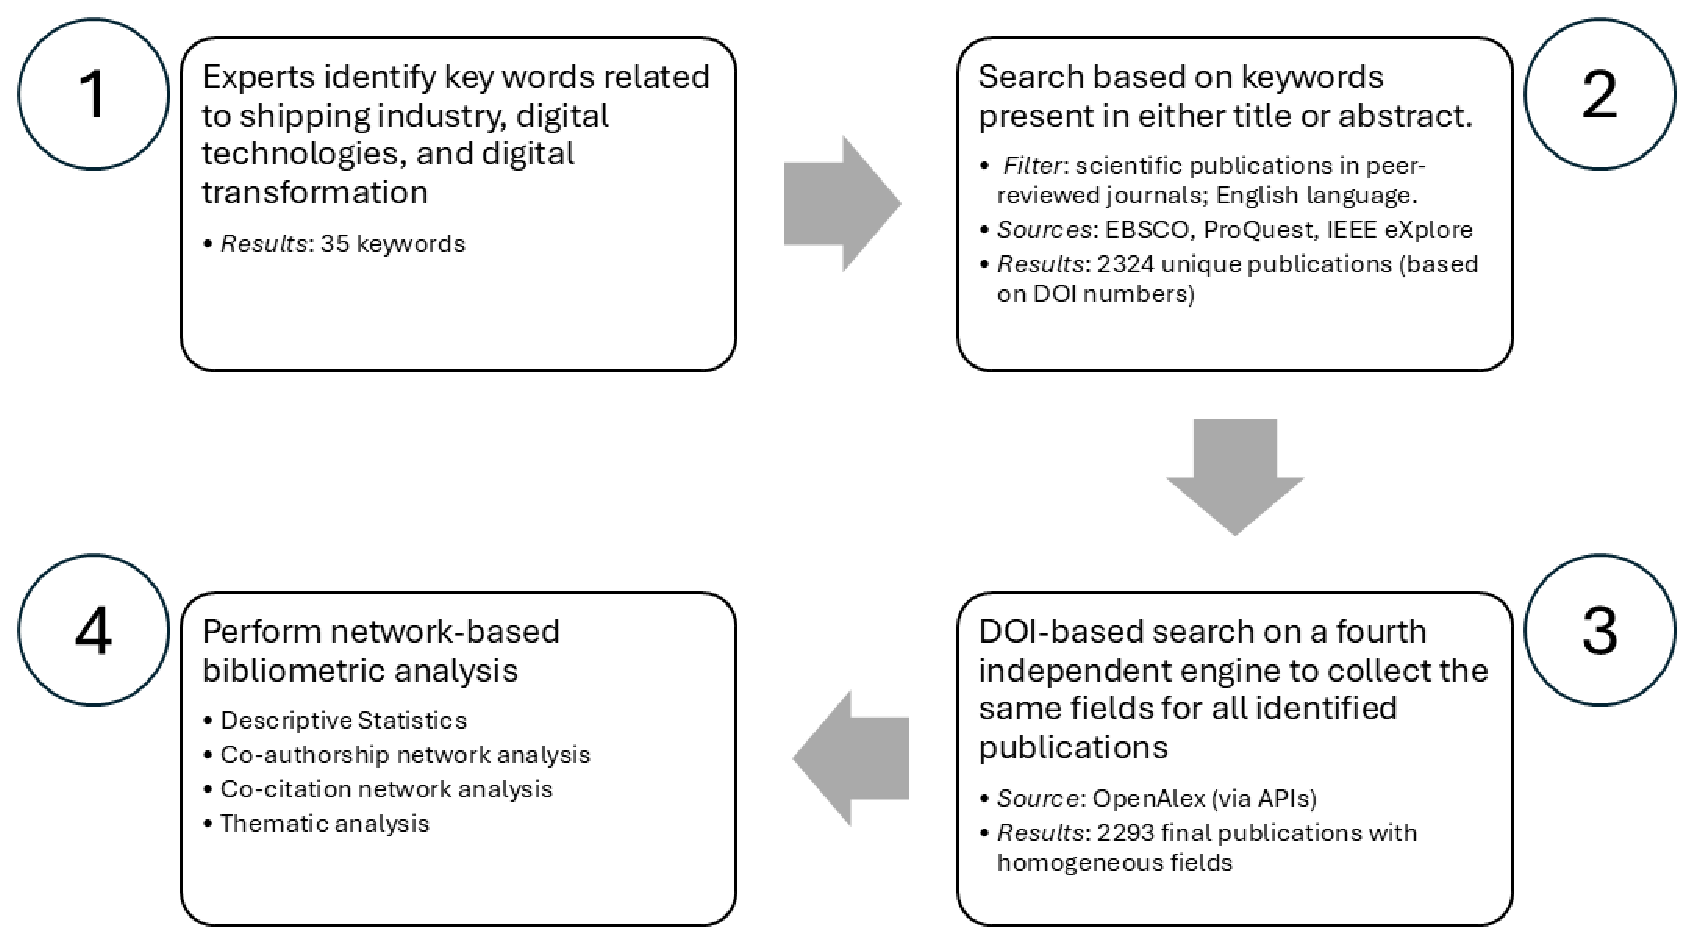
\includegraphics[width=\linewidth]{pics/overall_diagram.eps}
	\caption{Network-based bibliometric analysis diagram}\label{fig:fig0}
\end{figure}

\begin{figure}[H]
	\centering
	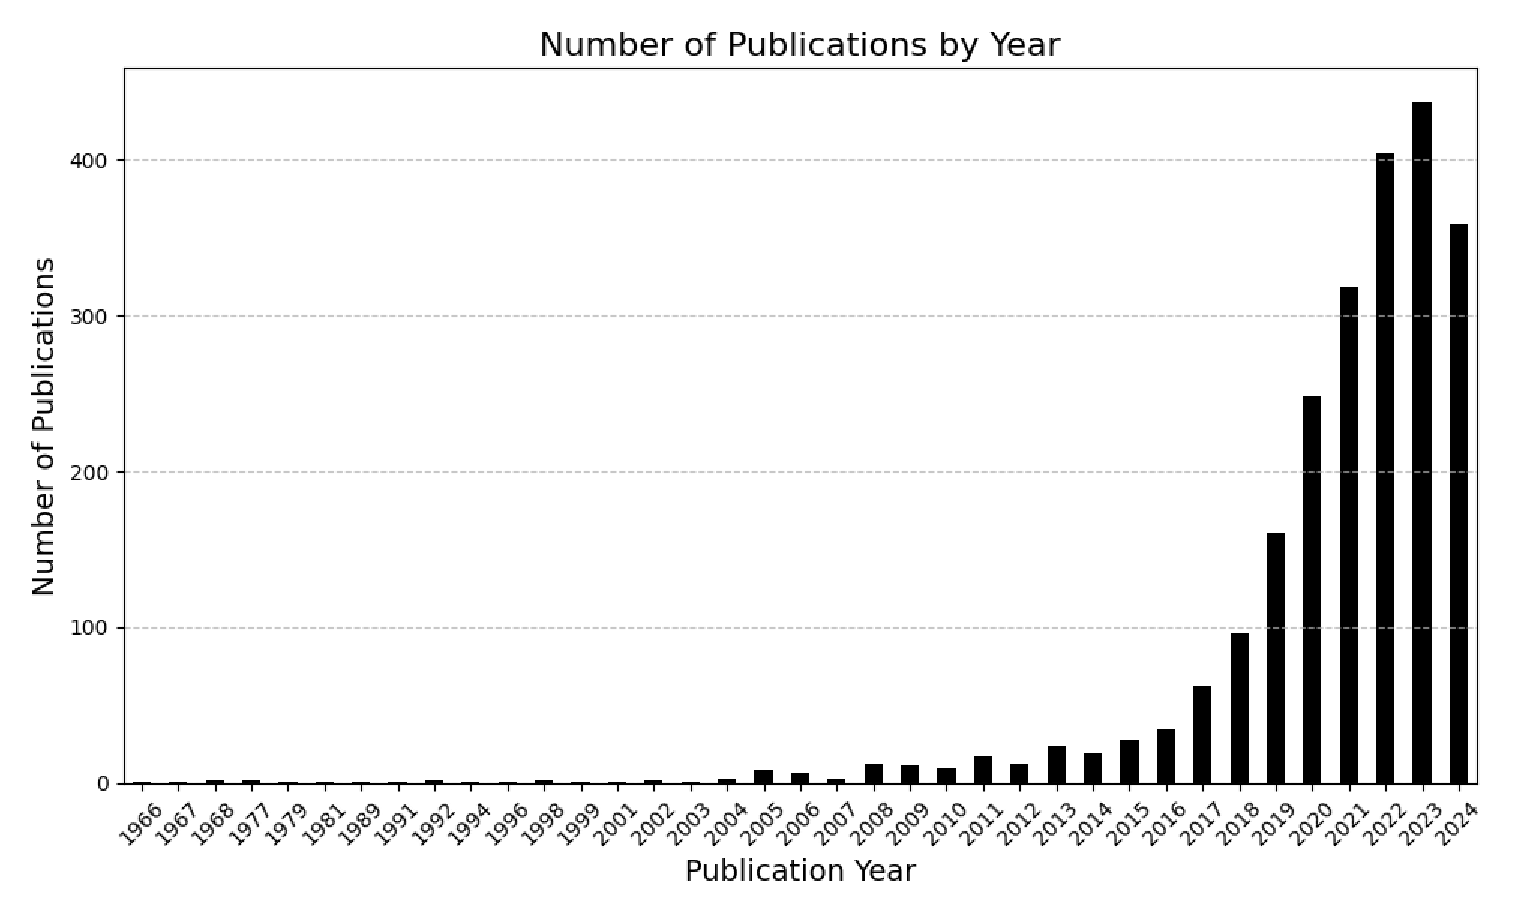
\includegraphics[width=\linewidth]{pics/no_publications_year.eps}
	\caption{Distribution of publications across years}\label{fig:fig1}
\end{figure}

\begin{figure}[H]
	\centering
	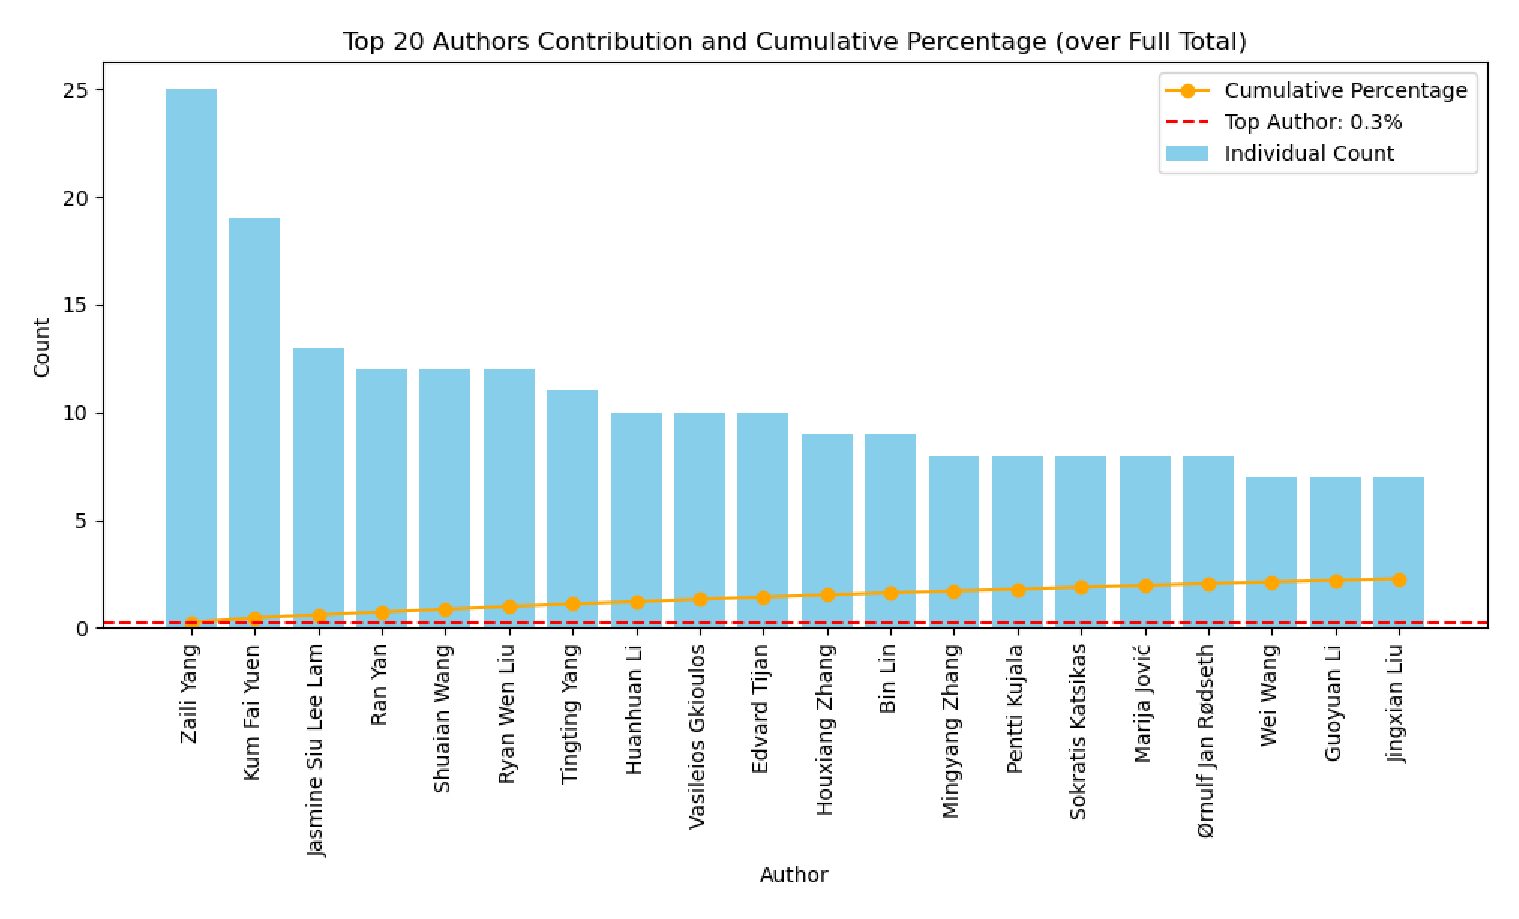
\includegraphics[height=0.3\textheight, keepaspectratio]{pics/leading_authors.eps}
	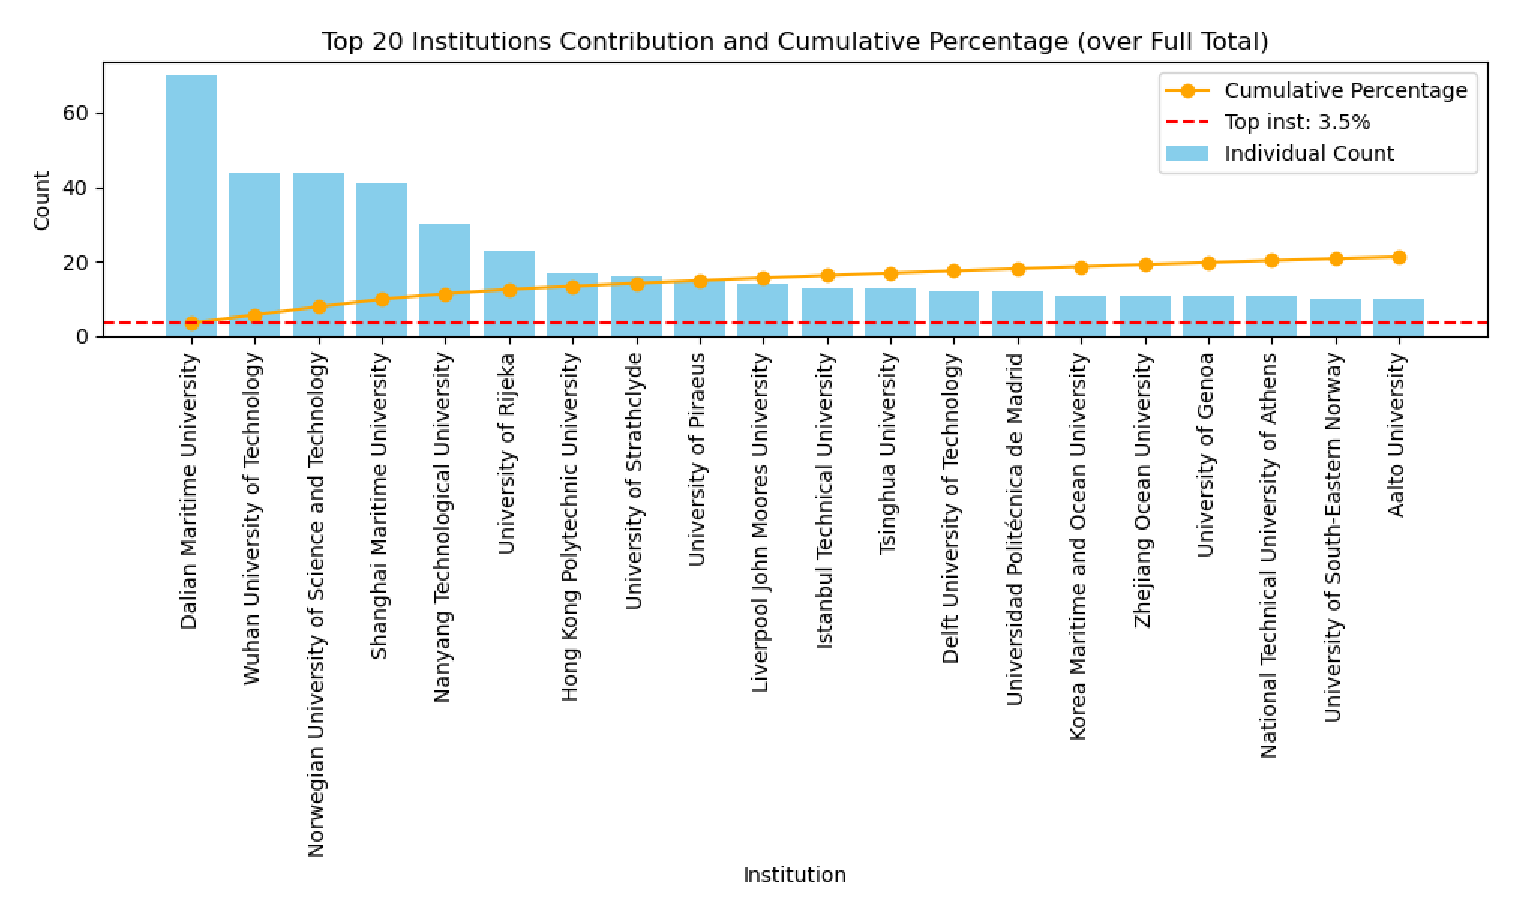
\includegraphics[height=0.3\textheight, keepaspectratio]{pics/leading_institutions.eps}
	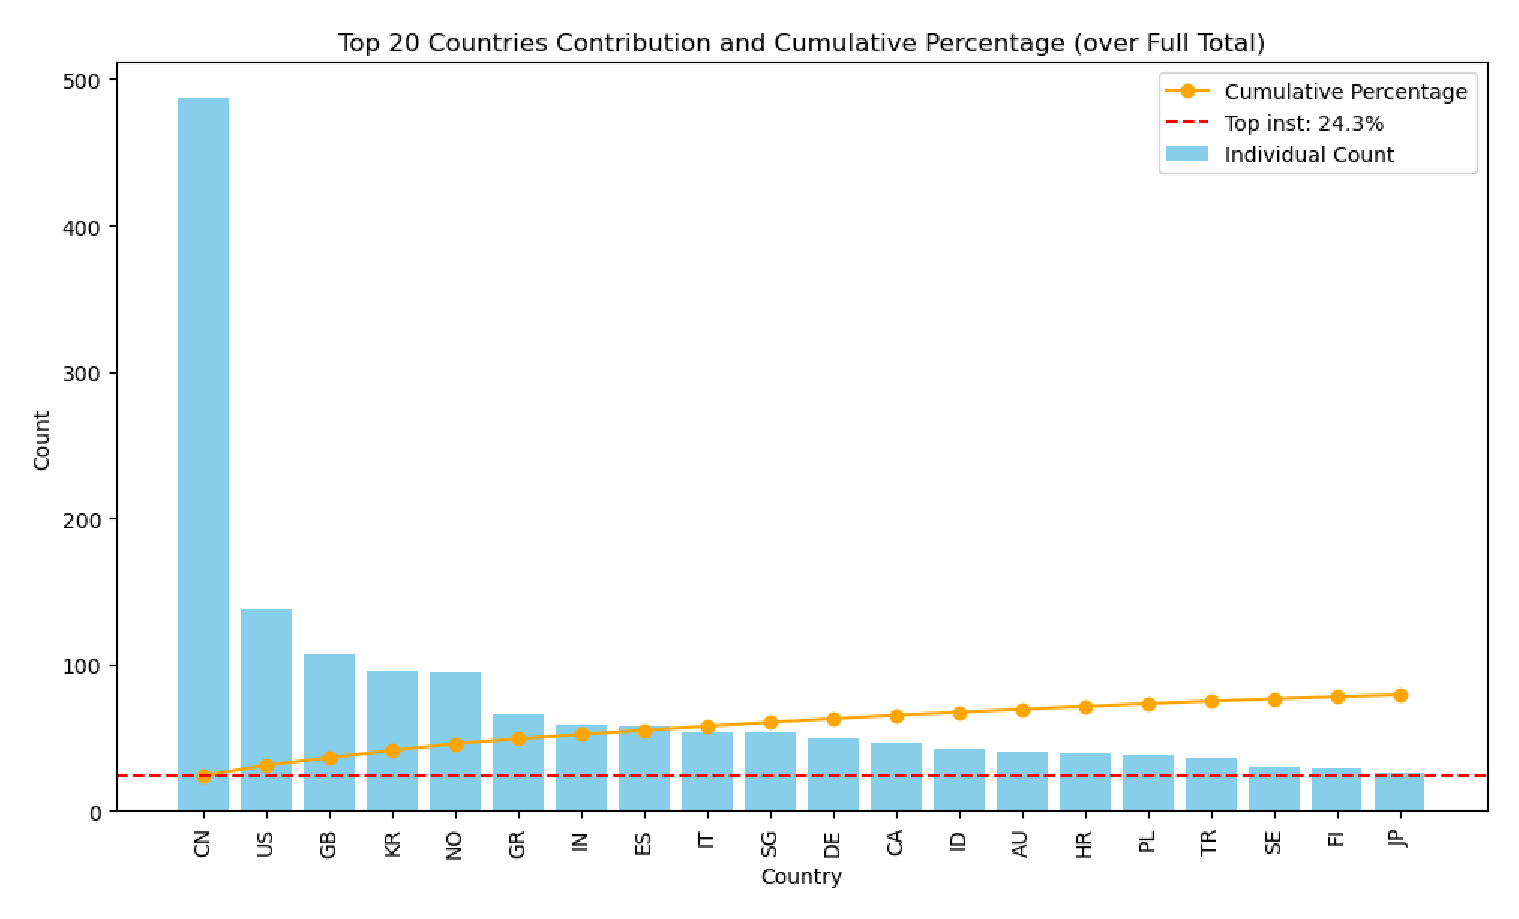
\includegraphics[height=0.3\textheight, keepaspectratio]{pics/leading_countries.eps}
	\caption{Top 20 leading authors (\textit{top}), institutions (\textit{middle}), and countries (\textit{bottom})}\label{fig:fig2}
\end{figure}

\begin{figure}[H]
	\centering
	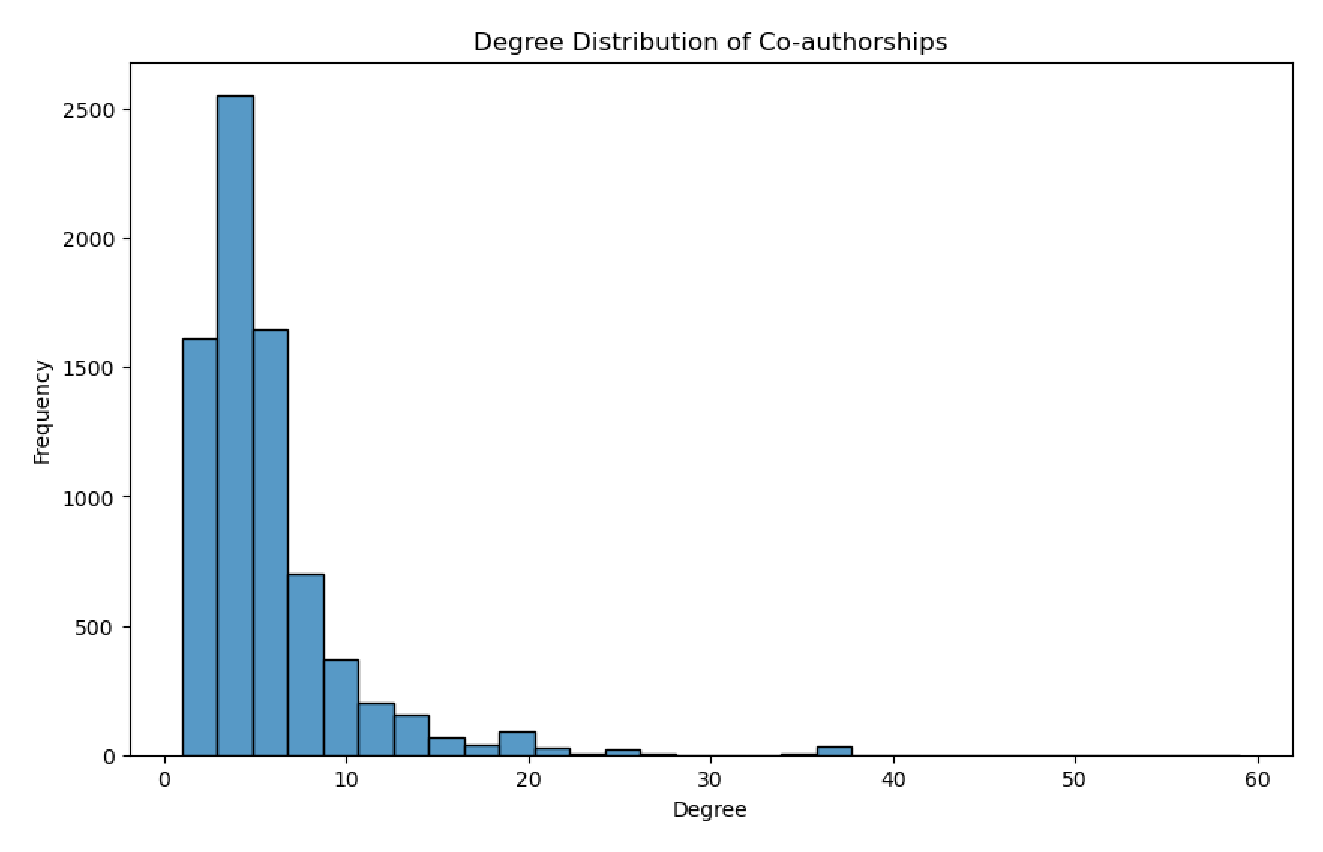
\includegraphics[height=0.2\textheight, keepaspectratio]{pics/coauthorship_degree_distribution.eps}
	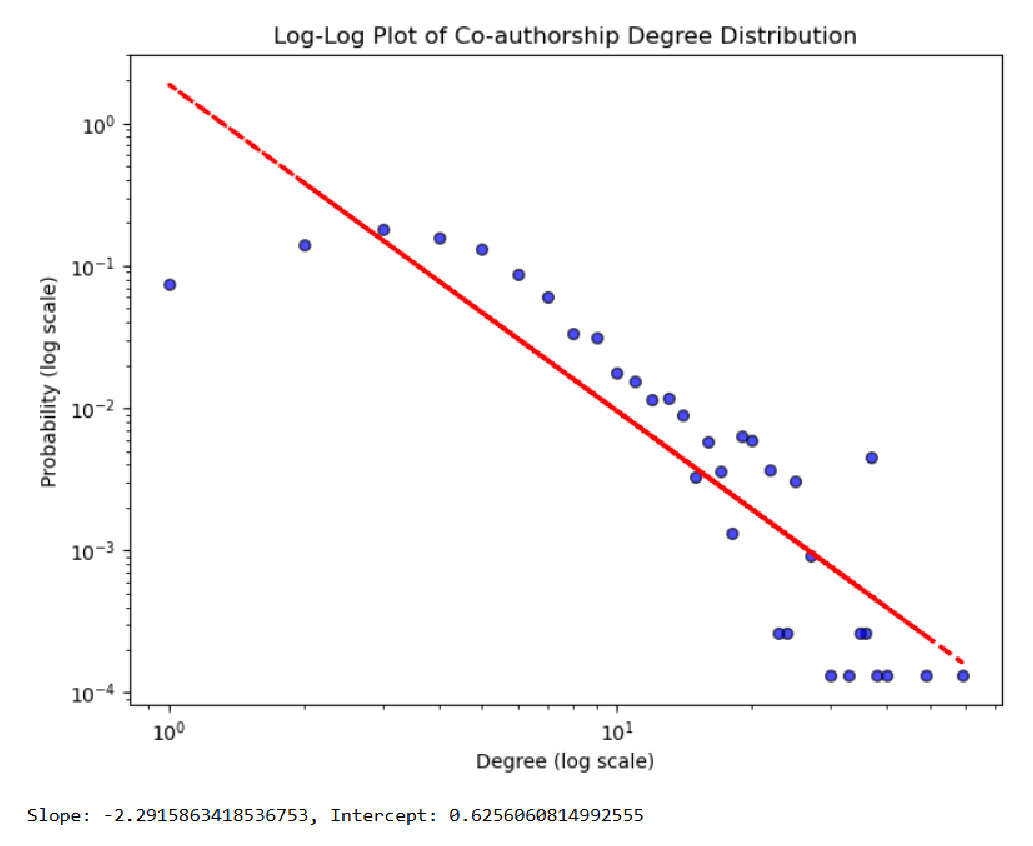
\includegraphics[height=0.2\textheight, keepaspectratio]{pics/coauthorship_degree_distribution_loglog_chart.eps}
	\caption{Co-authorship degree distribution (\textit{top}), and corresponding log-log chart (\textit{bottom})}\label{fig:fig3}
\end{figure}

\begin{figure}[H]
	\centering
	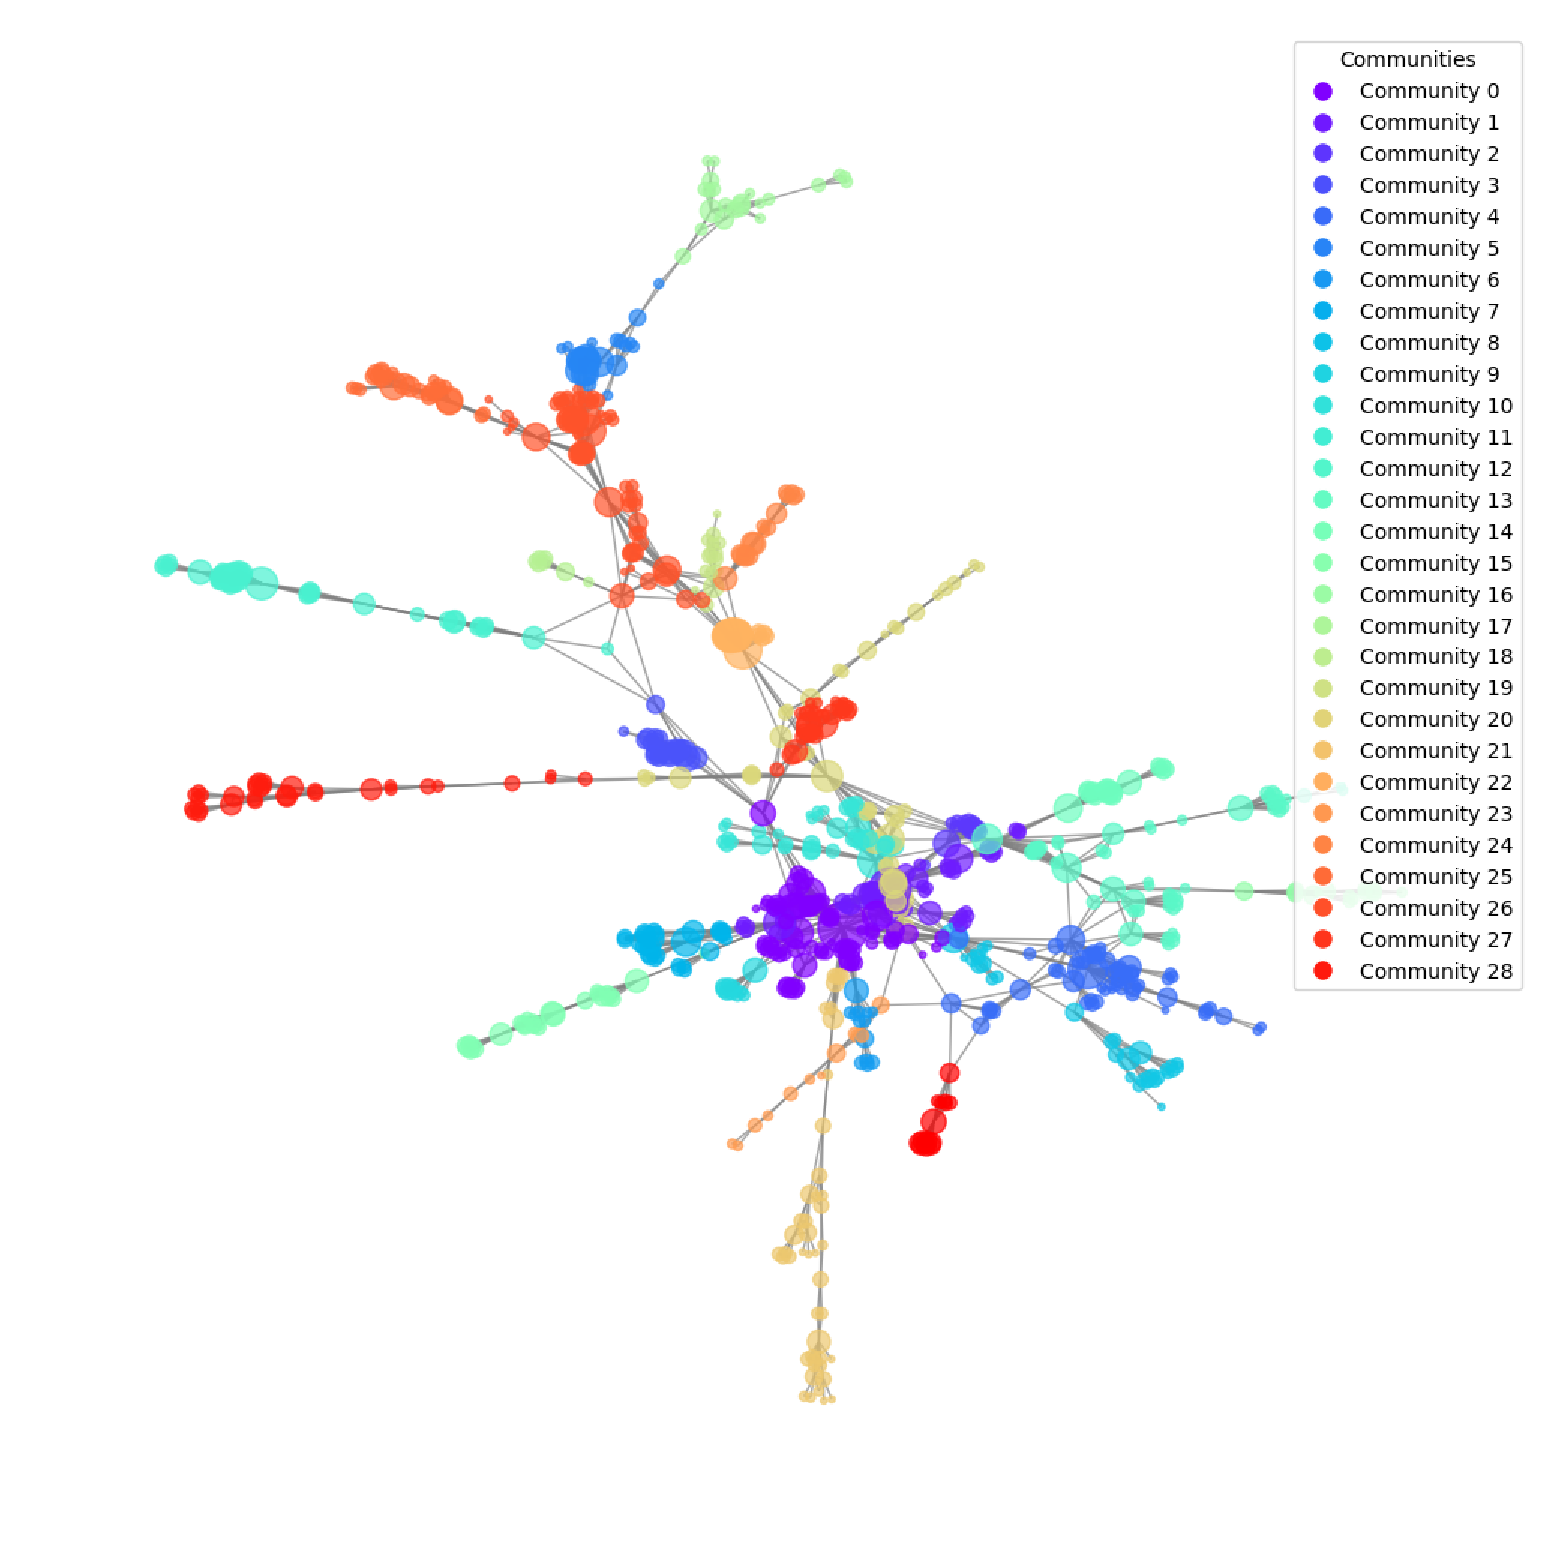
\includegraphics[width=\linewidth]{pics/co-authorship_communities.eps}
	\caption{Co-authorship network with communities}\label{fig:fig4}
\end{figure}

\begin{figure}[H]
	\centering
	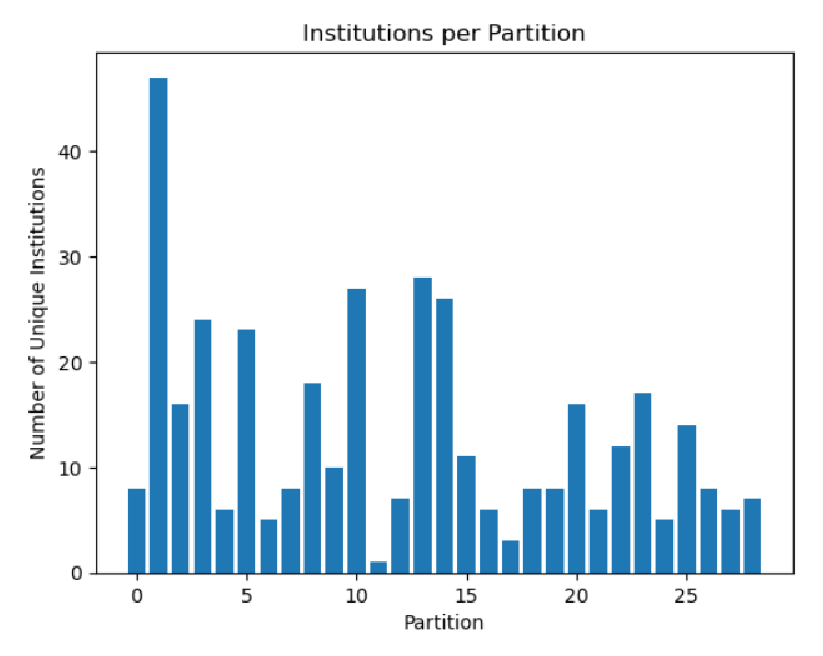
\includegraphics[height=0.2\textheight, keepaspectratio]{pics/coauthorship_inst_per_partition.eps}
	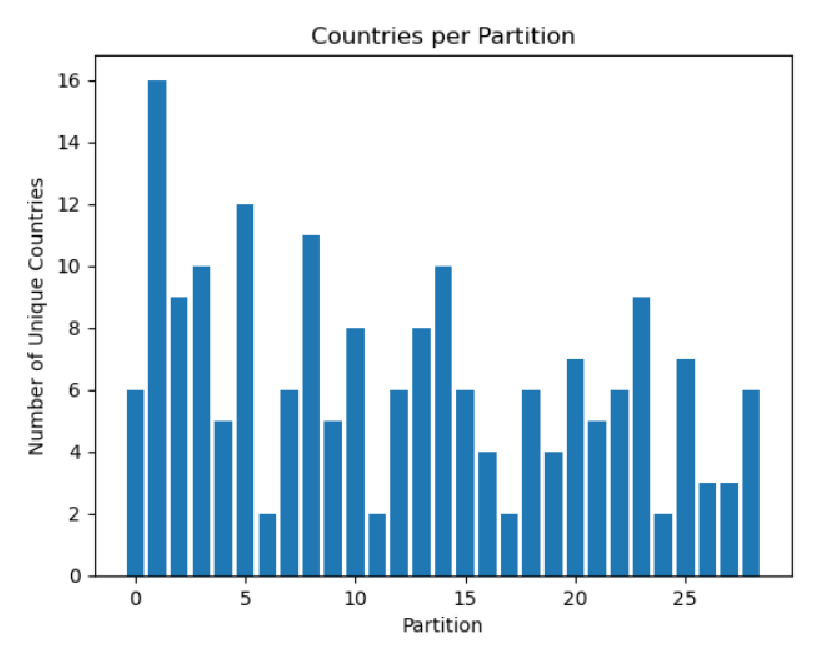
\includegraphics[height=0.2\textheight, keepaspectratio]{pics/coauthorship_country_per_partition.eps}
	\caption{Co-authorship distribution of institutions (\textit{top}) and countries (\textit{bottom}) across partitions}\label{fig:fig5}
\end{figure}

\begin{figure}[H]
	\centering
	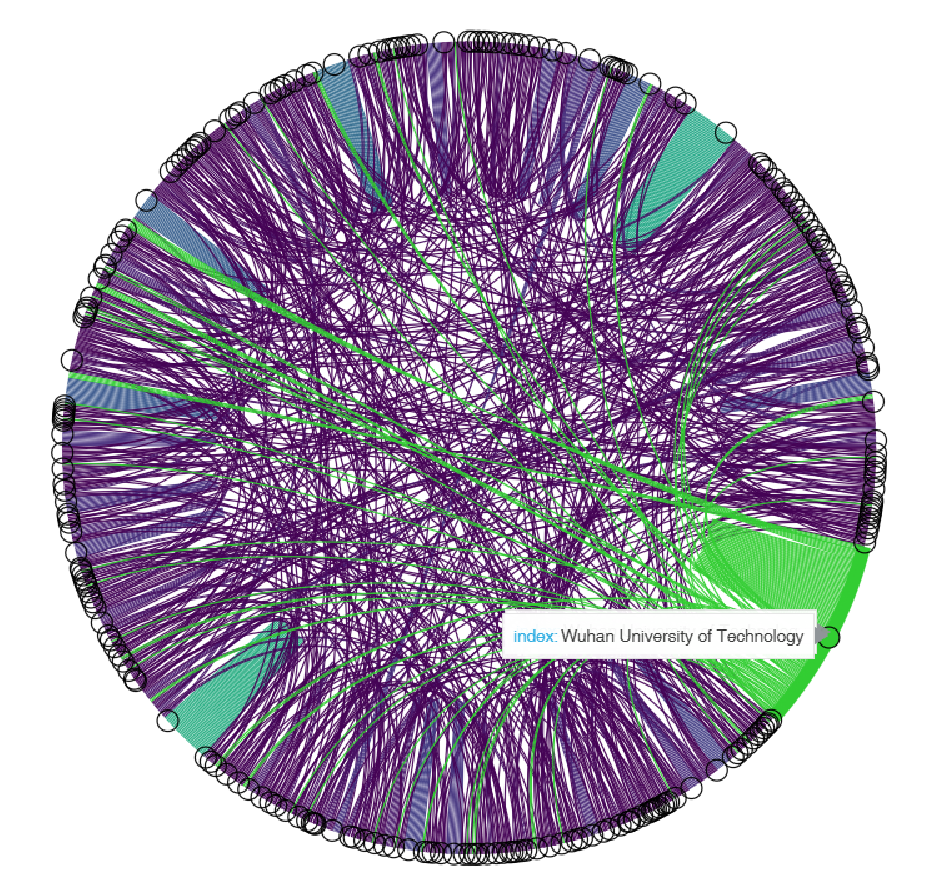
\includegraphics[height=0.3\textheight, keepaspectratio]{pics/coauthorship_inst_chord_1.eps}
	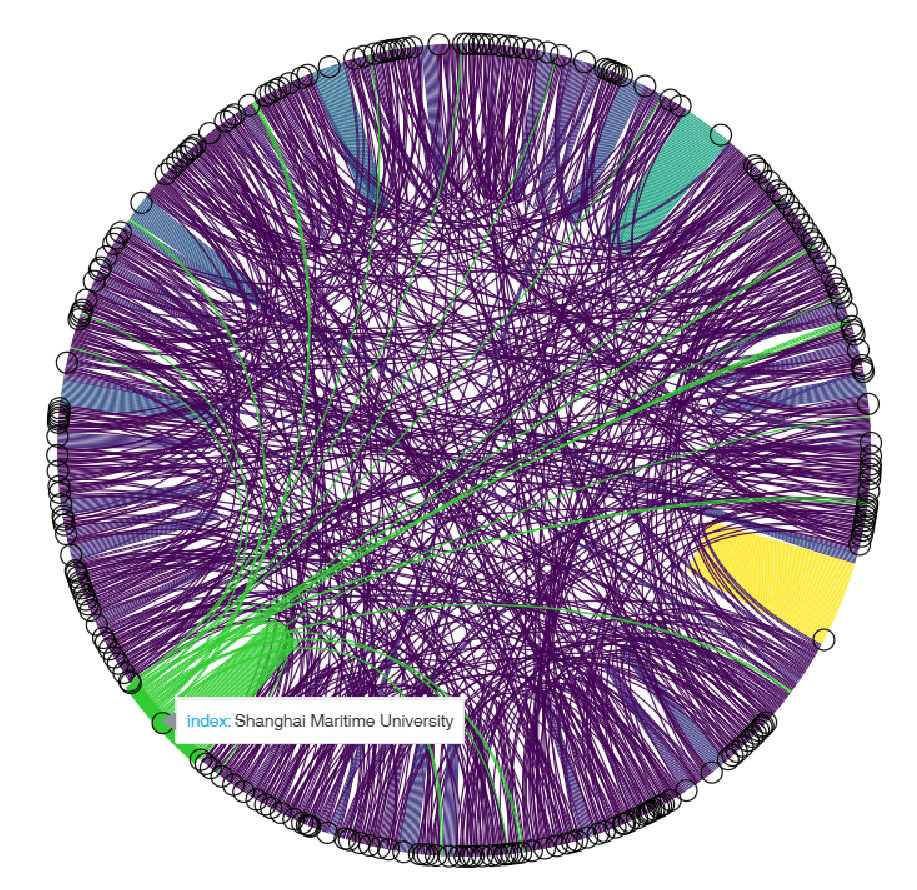
\includegraphics[height=0.3\textheight, keepaspectratio]{pics/coauthorship_inst_chord_2.eps}
	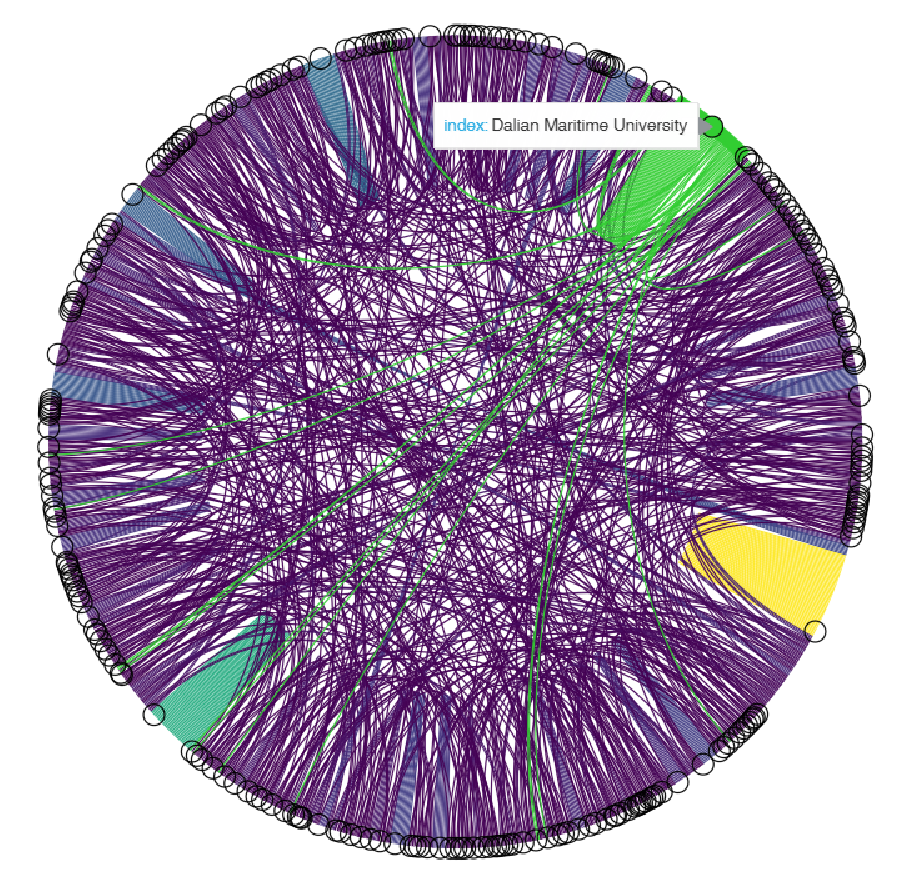
\includegraphics[height=0.3\textheight, keepaspectratio]{pics/coauthorship_inst_chord_3.eps}
	\caption{Chord diagrams for insitution mapping on co-authorship communities. The three diagrams show three relevant clusters: (\textit{top}) Wuhan University of Technology, (\textit{middle}) Shanghai Maritime University, and (\textit{bottom}) Dalian Maritime University}\label{fig:fig6}
\end{figure}

\begin{figure}[H]
	\centering
	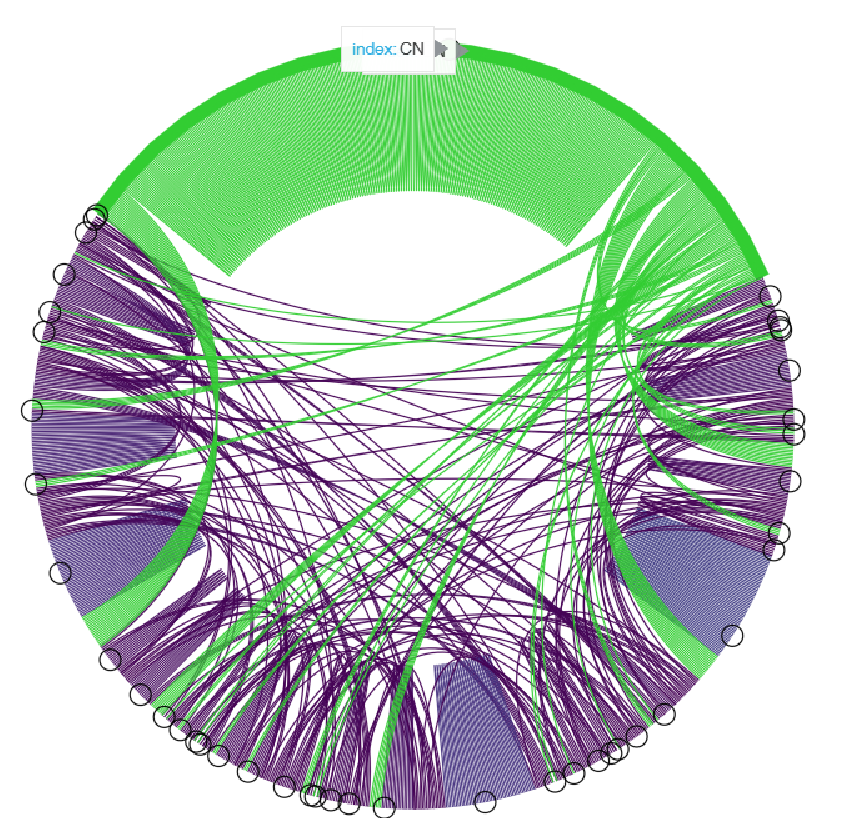
\includegraphics[height=0.3\textheight, keepaspectratio]{pics/coauthorship_country_chord_1.eps}
	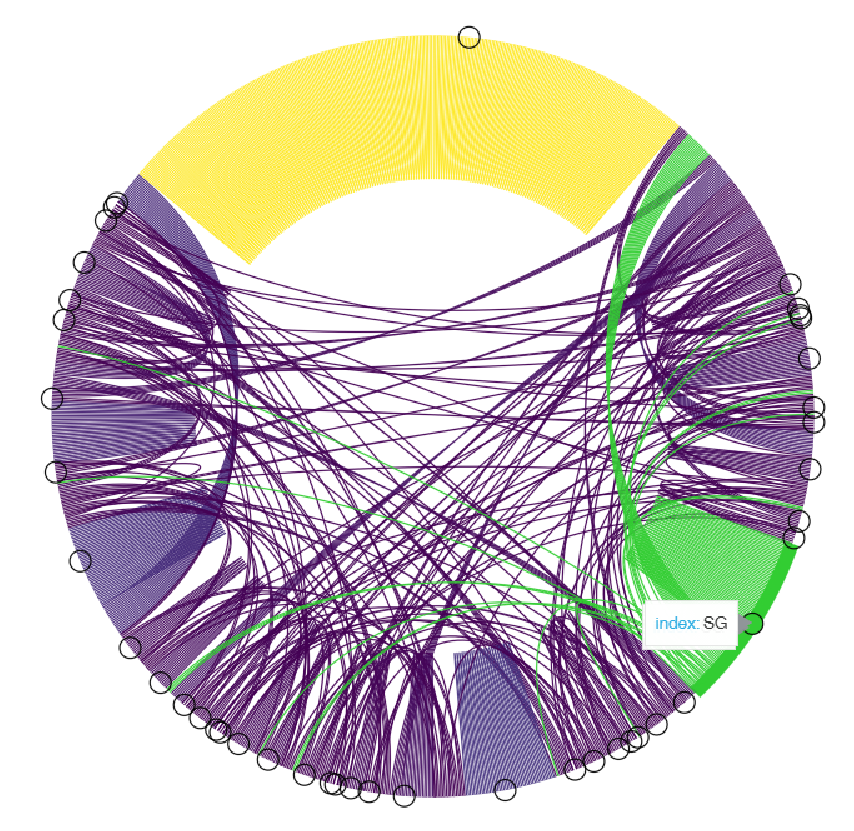
\includegraphics[height=0.3\textheight, keepaspectratio]{pics/coauthorship_country_chord_2.eps}
	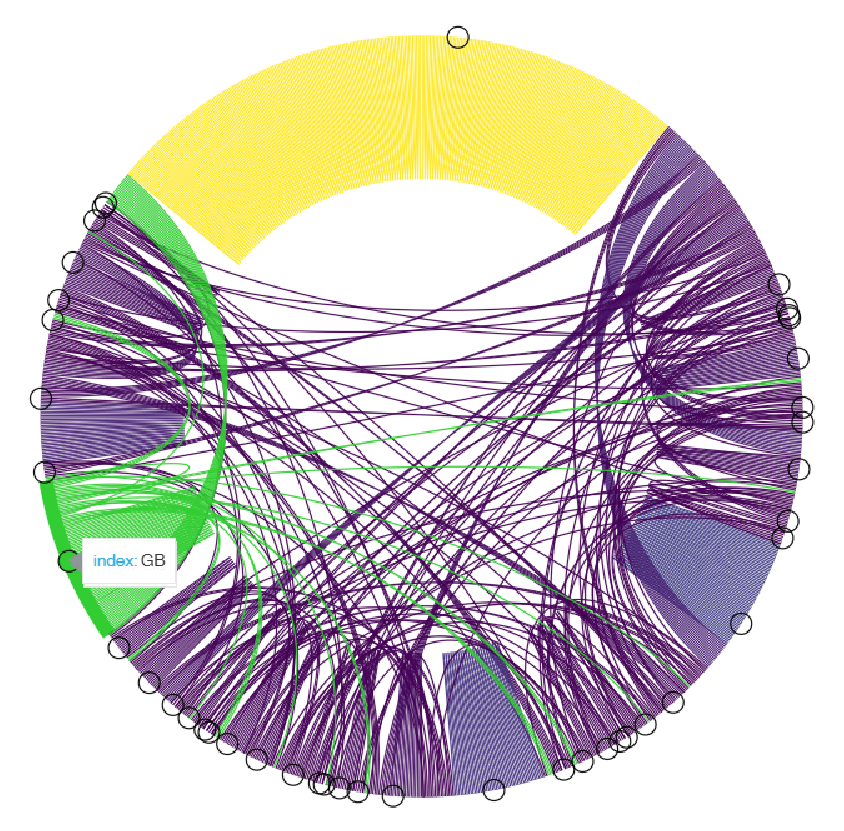
\includegraphics[height=0.3\textheight, keepaspectratio]{pics/coauthorship_country_chord_3.eps}
	\caption{Chord diagrams for countries mapping on co-authorship communities. The three diagrams show three relevant clusters:(\textit{top}) China, (\textit{middle}) Singapore, and (\textit{bottom}) Great Britain}\label{fig:fig7}
\end{figure}

\begin{figure}[H]
	\centering
	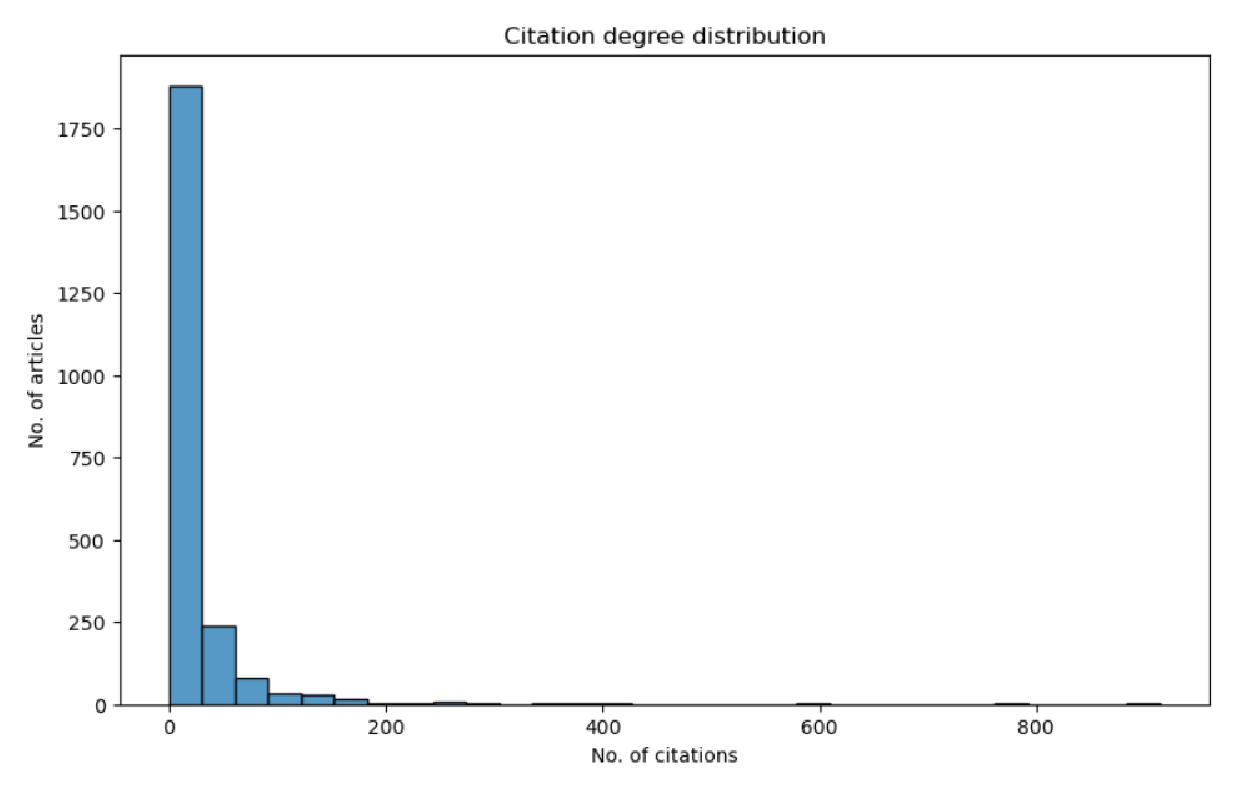
\includegraphics[height=0.2\textheight, keepaspectratio]{pics/citation_degree_distribution.eps}
	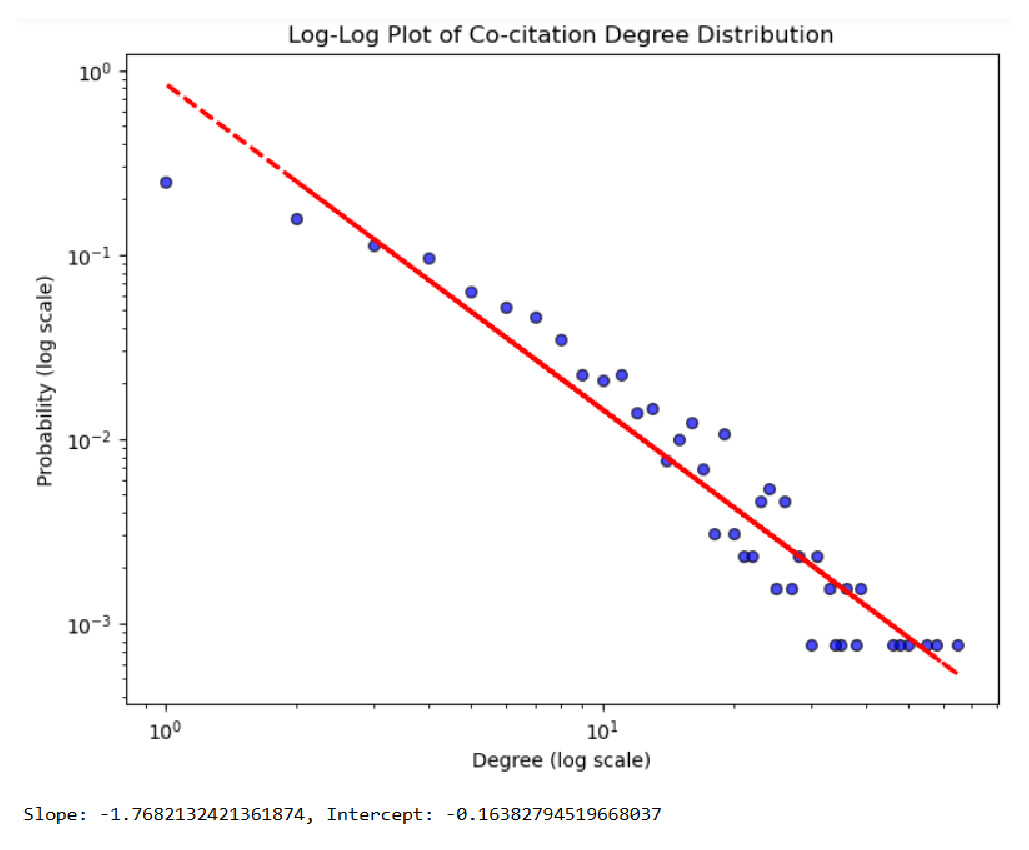
\includegraphics[height=0.2\textheight, keepaspectratio]{pics/loglog_citation_degree_distribution.eps}
	\caption{Co-citation degree distribution and log-log chart} \label{fig:fig8}
\end{figure}

\begin{figure}[H]
	\centering
	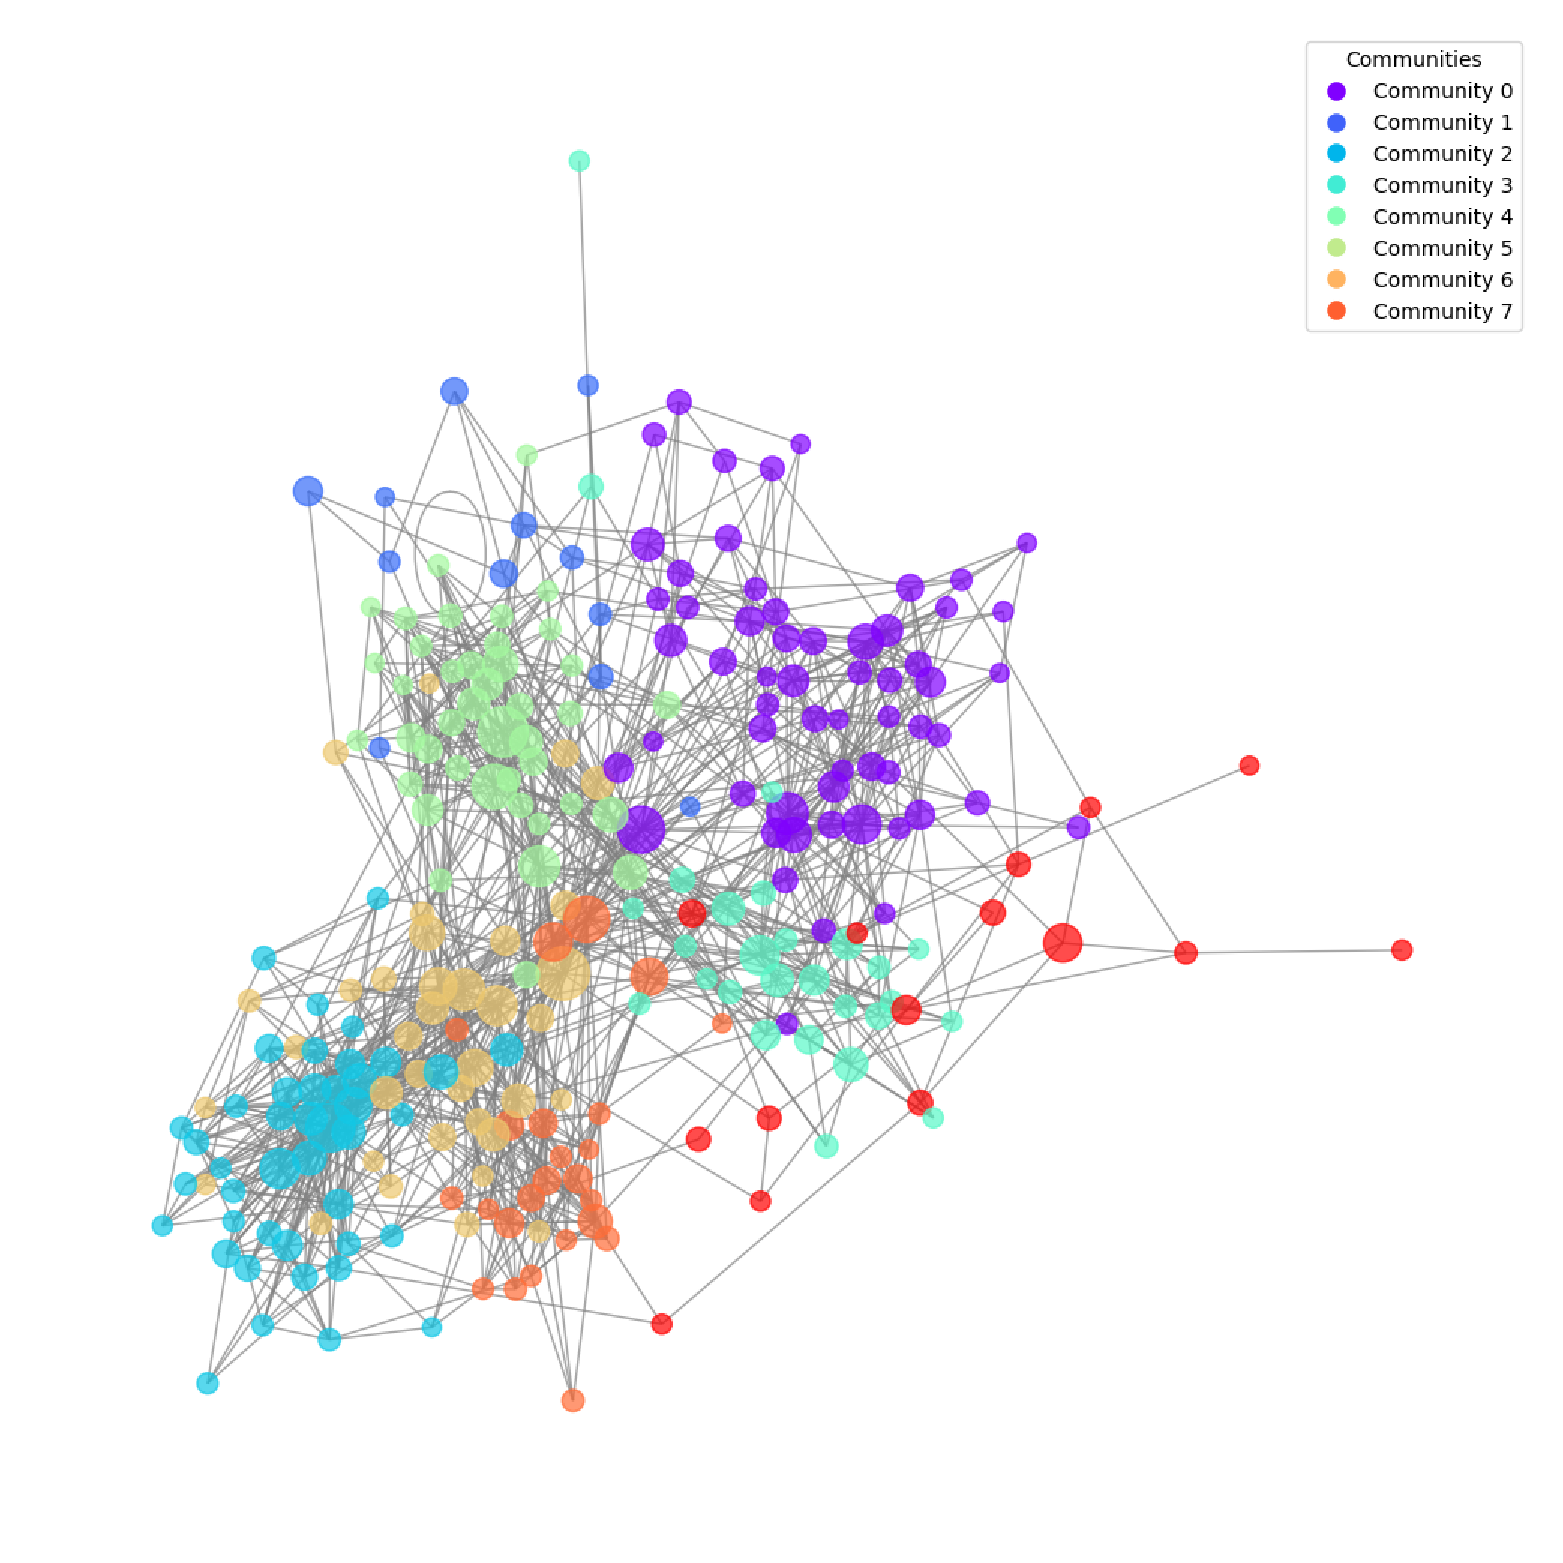
\includegraphics[width=\linewidth]{pics/cocitation_communiities.eps}
	\caption{Co-citation network with communities}\label{fig:fig9}
\end{figure}

\begin{figure}[H]
	\centering
	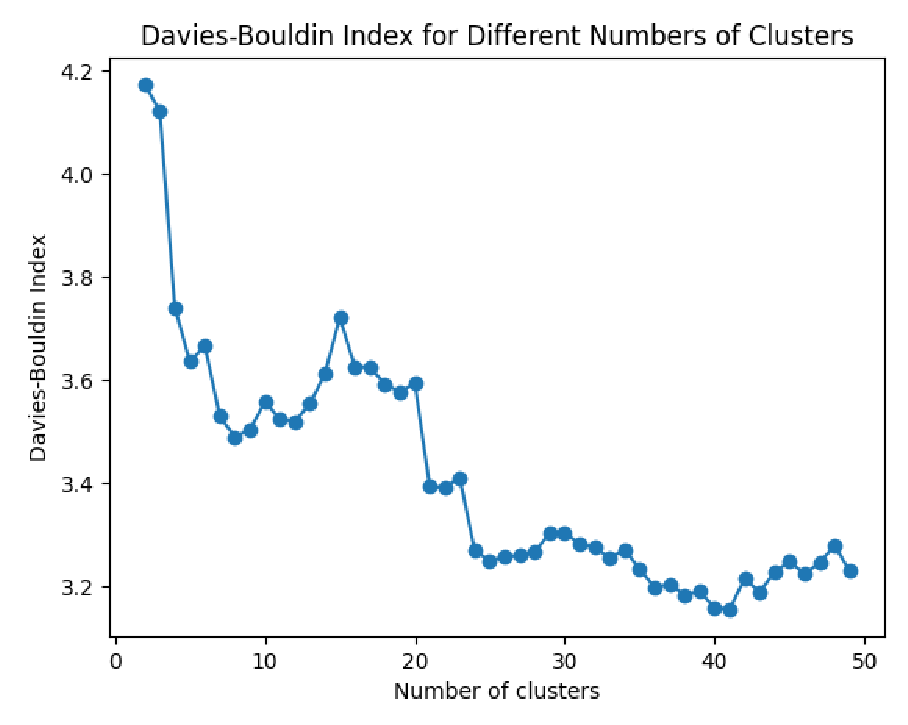
\includegraphics[height=0.2\textheight, keepaspectratio]{pics/davis_bouldin.eps}
	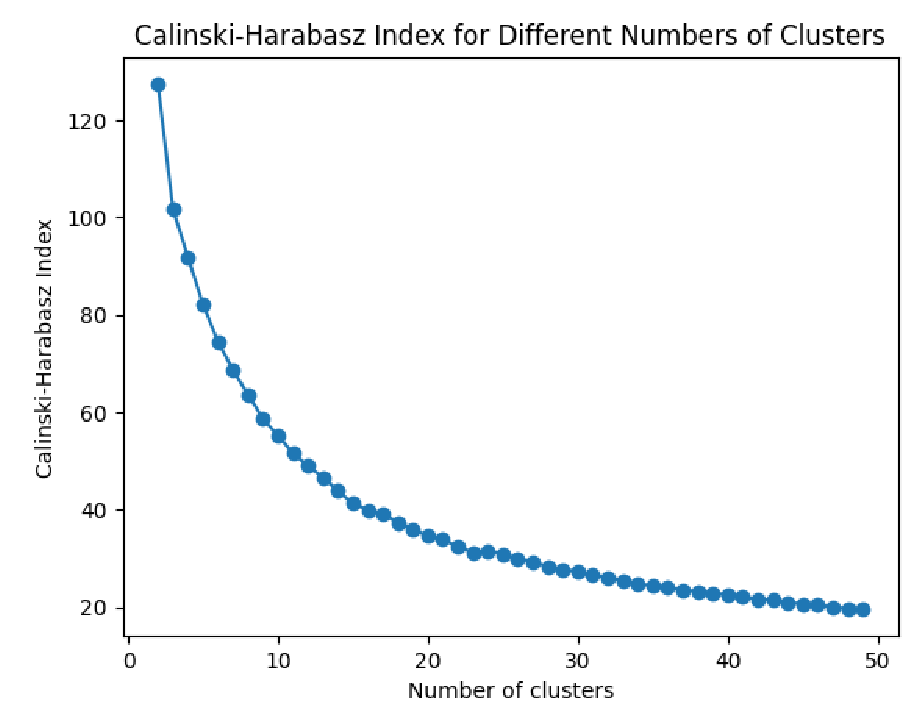
\includegraphics[height=0.2\textheight, keepaspectratio]{pics/calinski.eps}
	\caption{Davies-Bouldin (\text{top}) and Calinski-Harabasz (\textit{bottom}) indexes.}\label{fig:fig10}
\end{figure}

\begin{figure}[H]
	\centering
	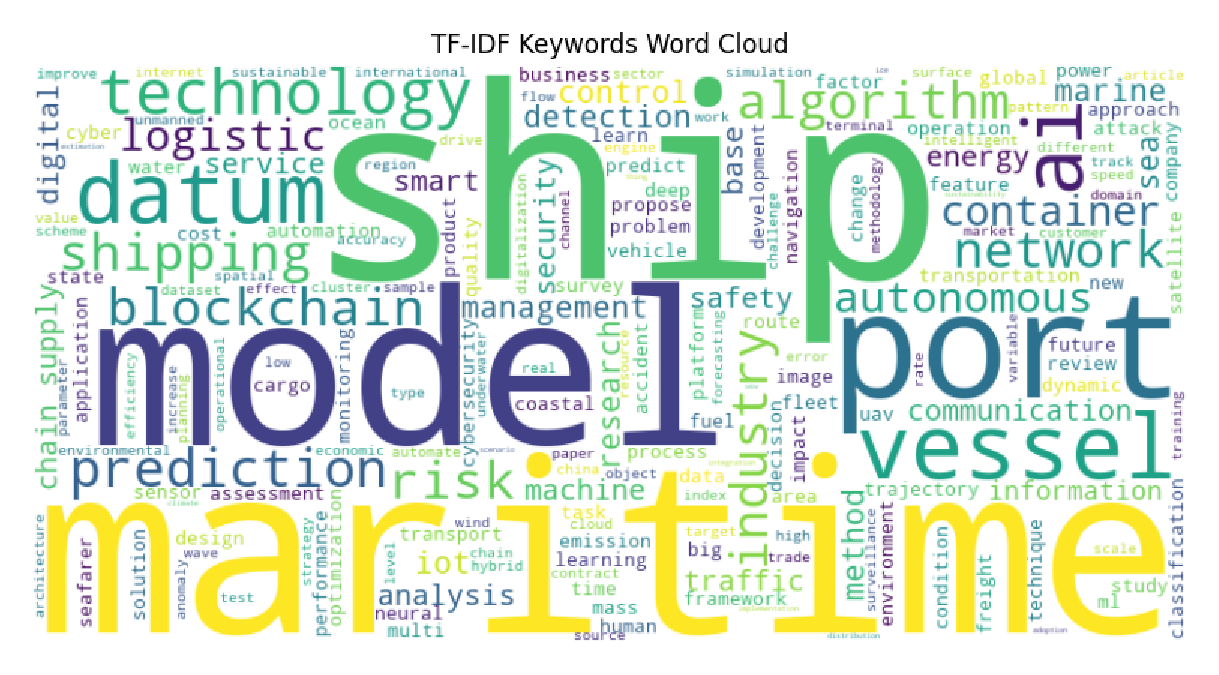
\includegraphics[width=\linewidth]{pics/wordcloud_1.eps}
	\caption{Word cloud based on TF-IDF}\label{fig:fig11}
\end{figure}

\begin{figure}[H]
	\centering
	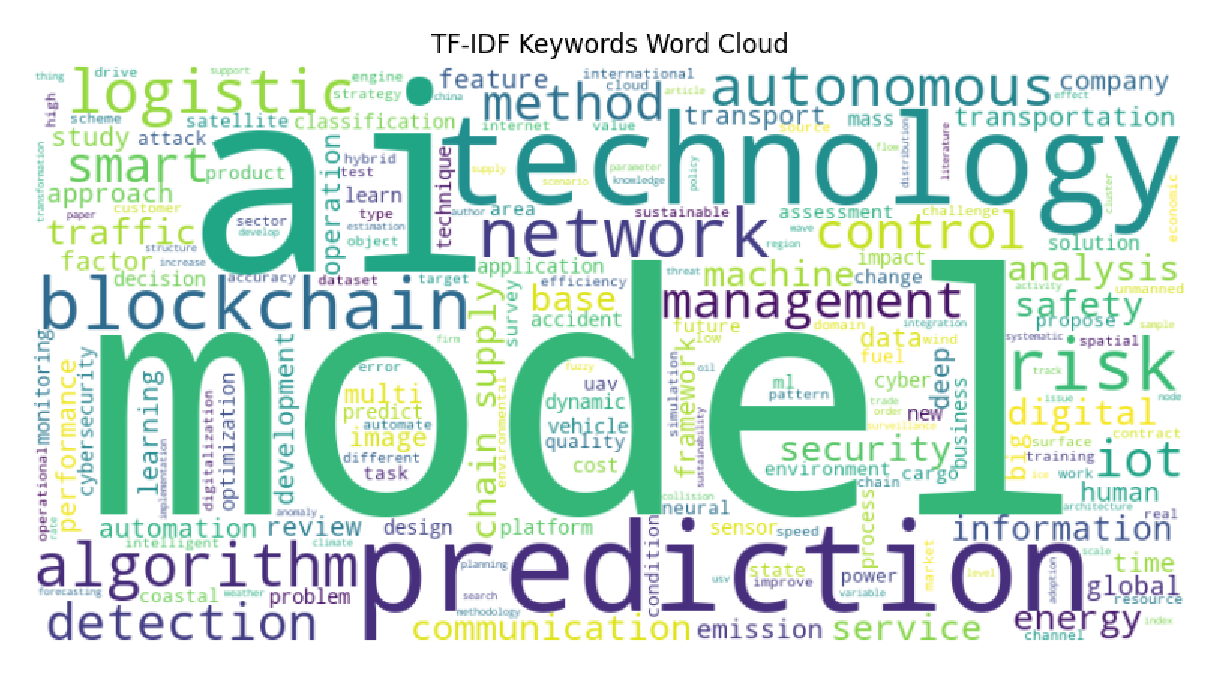
\includegraphics[width=\linewidth]{pics/wordcloud_2.eps}
	\caption{Word cloud focused on technological terms}\label{fig:fig12}
\end{figure}

\begin{figure}[H]
	\centering
	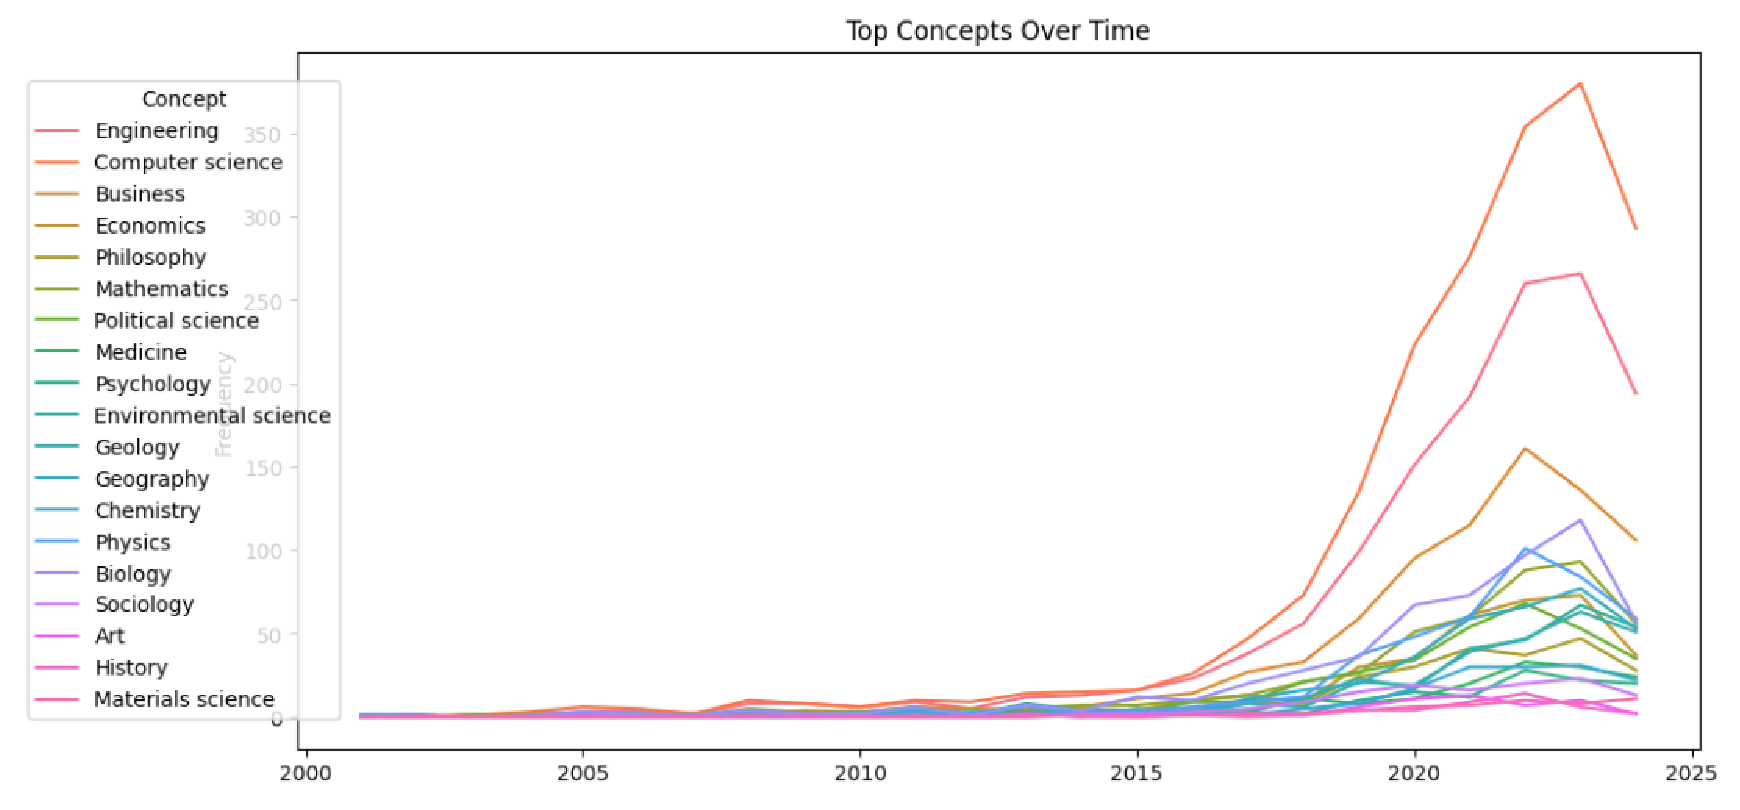
\includegraphics[width=\linewidth]{pics/main_concept_trend_toplevel.eps}
	\caption{Top-level OpenAlex concept distribution over time terms}\label{fig:fig13}
\end{figure}

\begin{figure}[H]
	\centering
	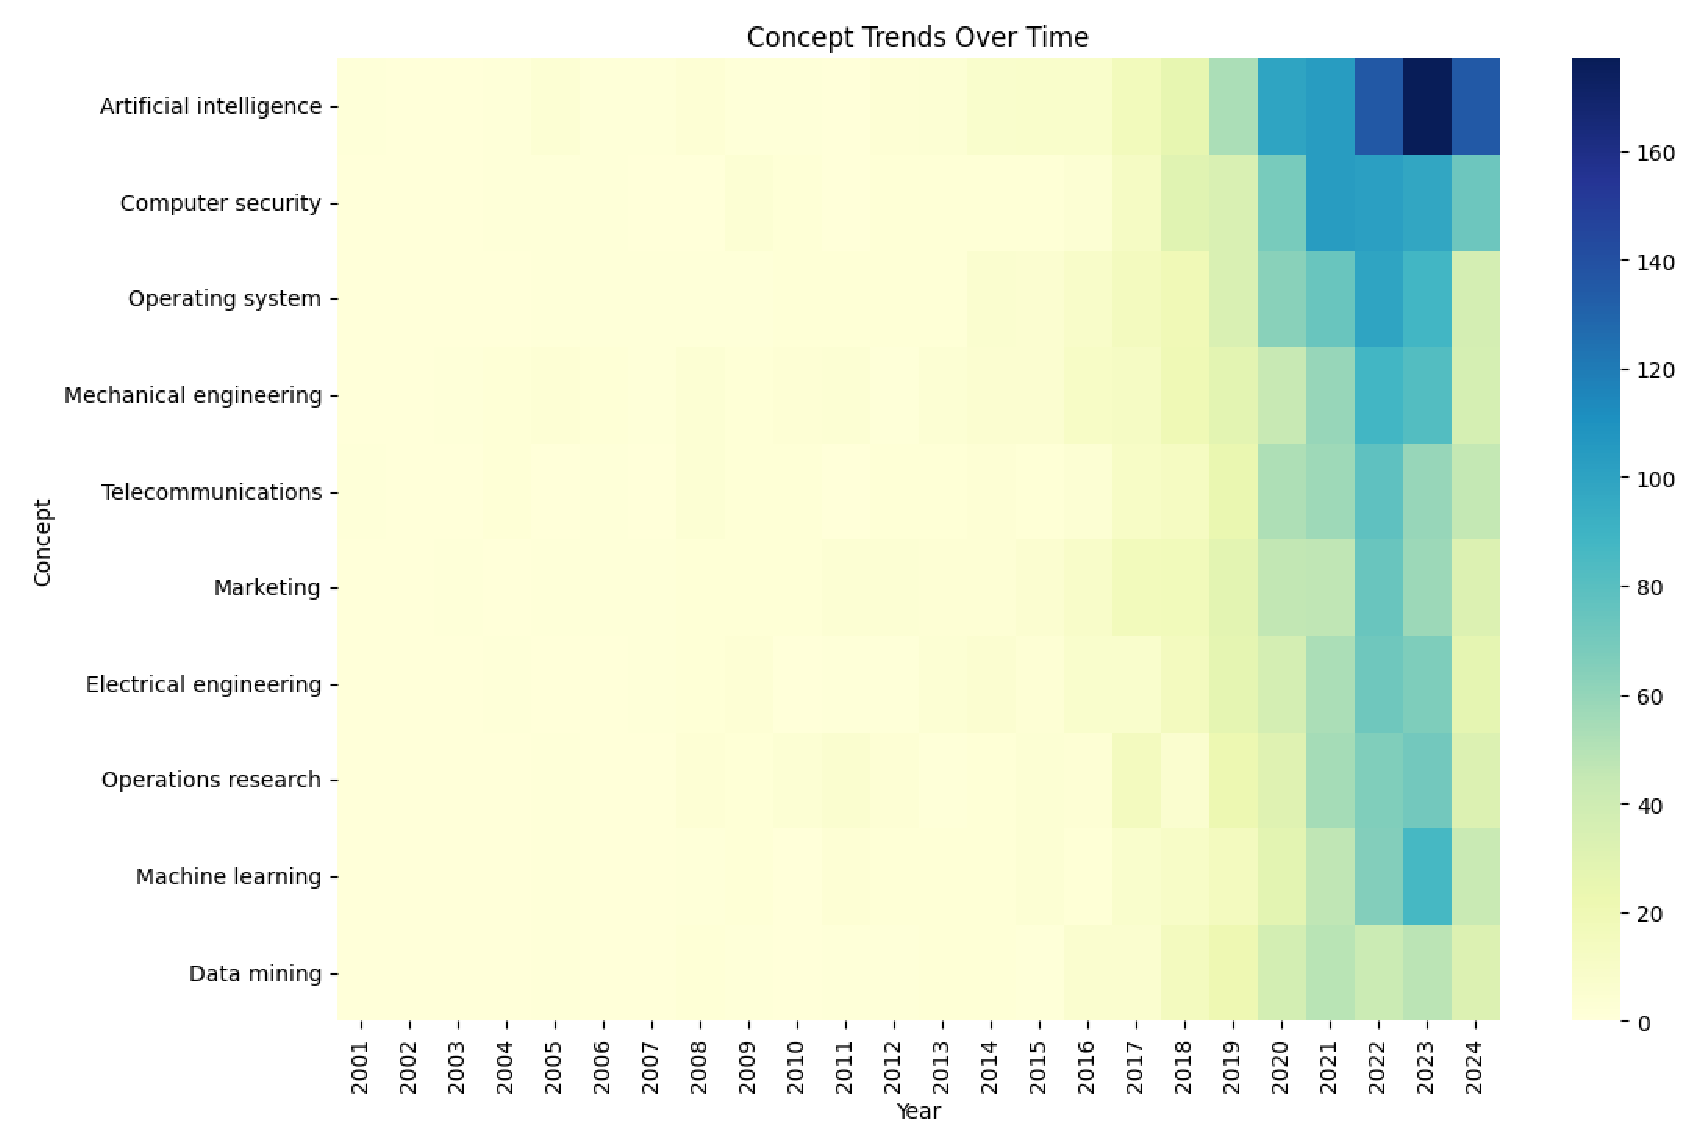
\includegraphics[width=\linewidth]{pics/main_concept_trend_lowerlevels.eps}
	\caption{Detail-level OpenAlex concept distribution over time for the 10 most relevant terms}\label{fig:fig14}
\end{figure}

% If authors have biography, please use the format below
%\section*{Short Biography of Authors}
%\bio
%{\raisebox{-0.35cm}{\includegraphics[width=3.5cm,height=5.3cm,clip,keepaspectratio]{Definitions/author1.pdf}}}
%{\textbf{Firstname Lastname} Biography of first author}
%
%\bio
%{\raisebox{-0.35cm}{\includegraphics[width=3.5cm,height=5.3cm,clip,keepaspectratio]{Definitions/author2.jpg}}}
%{\textbf{Firstname Lastname} Biography of second author}

% For the MDPI journals use author-date citation, please follow the formatting guidelines on http://www.mdpi.com/authors/references
% To cite two works by the same author: \citeauthor{ref-journal-1a} (\citeyear{ref-journal-1a}, \citeyear{ref-journal-1b}). This produces: Whittaker (1967, 1975)
% To cite two works by the same author with specific pages: \citeauthor{ref-journal-3a} (\citeyear{ref-journal-3a}, p. 328; \citeyear{ref-journal-3b}, p.475). This produces: Wong (1999, p. 328; 2000, p. 475)

%%%%%%%%%%%%%%%%%%%%%%%%%%%%%%%%%%%%%%%%%%
%% for journal Sci
%\reviewreports{\\
%Reviewer 1 comments and authors’ response\\
%Reviewer 2 comments and authors’ response\\
%Reviewer 3 comments and authors’ response
%}
%%%%%%%%%%%%%%%%%%%%%%%%%%%%%%%%%%%%%%%%%%
\PublishersNote{}
%\isPreprints{} % If the paper is ``preprints'', please uncomment this parenthesis.
\end{document}

